\section{Preventivo} %Meccanismi di controllo e rendicontazione
Viene in seguito presentato il preventivo del costo del lavoro da svolgere con i dettagli sul costo di ogni singolo periodo.
Per identificare i diversi ruoli verranno utilizzate le sigle:
\begin{itemize}
	\item \textbf{Re}: responsabile di progetto\glo;
	\item \textbf{Am}: amministratore di progetto\glo;
	\item \textbf{An}: analista;
	\item \textbf{Pt}: progettista;
	\item \textbf{Pr}: programmatore;
	\item \textbf{Ve}: verificatore.
\end{itemize}
	\subsection{Periodo di analisi}
	Le ore indicate per questo periodo vengono riportate solo perché utili ai fini del documento, non saranno rendicontate nel budget finale richiesto in quanto il periodo di analisi è da considerare come investimento per il gruppo.
	\pagebreak
		\subsubsection{Prospetto orario}
		Nel periodo di analisi è prevista la seguente divisione oraria:
		\begin{longtable} {				
				>{}p{40mm}  
				>{}p{8mm}
				>{}p{8mm}
				>{}p{8mm}
				>{}p{8mm}
				>{}p{8mm}
				>{}p{8mm}
				>{}p{12mm}				
			}			
			\rowcolor{gray!50}
			\textbf{Nominativo} & \textbf{Re} & \textbf{Am} & \textbf{An} & \textbf{Pt} & \textbf{Pr} & \textbf{Ve} & \textbf{Totale}	\TBstrut \\ [2mm]
			Corrizzato Vittorio & 6 & 6 & 8 & - & - & 5 & 25 \TBstrut \\ [2mm]
			Dalla Libera Marco & 7 & - & 13 & - & - & 5 & 25 \TBstrut \\ [2mm]
			Rampazzo Marco & - & 8 & 12 & - & - & 5 & 25 \TBstrut \\ [2mm]
			Santagiuliana Vittorio & - & 5 & 12 & - & - & 8 & 25 \TBstrut \\ [2mm]
			Schiavon Rebecca & - & - & 15 & - & - & 10 & 25 \TBstrut \\ [2mm]
			Spreafico Alessandro & - & - & 12 & 5 & - & 8 & 25 \TBstrut \\ [2mm]
			Toffoletto Massimo & 8 & 7 & 5 & - & - & 5 & 25 \TBstrut \\ [2mm]
			\rowcolor{white}
			\caption{Prospetto orario del periodo di analisi}
		\end{longtable}
		Rappresentata nel seguente grafico:
		\begin{figure} [H]
			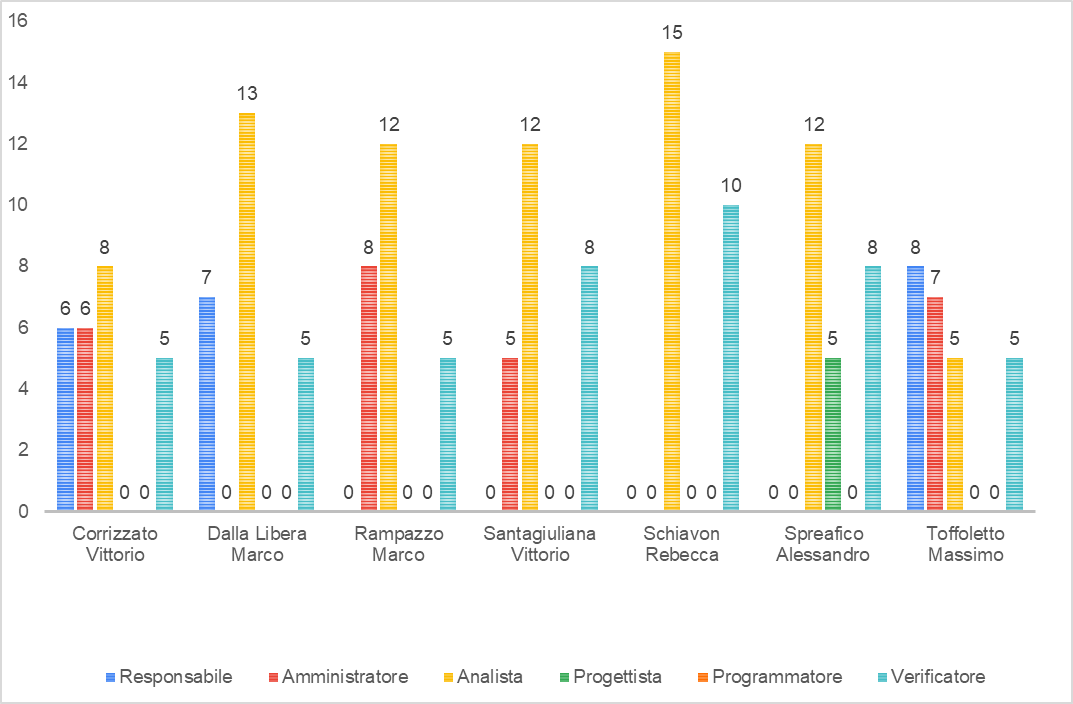
\includegraphics[width=\linewidth]{./img/Grafici/1.png}
			\caption{Grafico del prospetto orario del periodo di analisi}
		\end{figure}
	
		\subsubsection{Prospetto economico}
		Nel periodo di analisi sono previsti i seguenti costi:
		\begin{longtable} {
			>{}p{32mm}
			>{}p{20mm}
			>{}p{20mm}
		}
		\rowcolor{gray!50}
		
		\textbf{Ruolo} & \textbf{Ore} & \textbf{Costo} \TBstrut \\
		Responsabile & 21 & 630,00\euro{} \TBstrut \\
		Amministratore & 26 & 520,00\euro{} \TBstrut \\
		Analista & 77 & 1925,00\euro{} \TBstrut \\
		Progettista & 5 & 110,00\euro{} \TBstrut \\
		Programmatore & 0 & 0,00\euro{} \TBstrut \\
		Verificatore & 46 & 690,00\euro{} \TBstrut \\
		\textbf{Totale} & \textbf{175}& \textbf{3875,00\euro{}} \TBstrut \\
		\rowcolor{white}
		\caption{Prospetto economico del periodo di analisi}		
		\end{longtable}
		Rappresentati nel seguente grafico:
		\begin{figure} [H]
			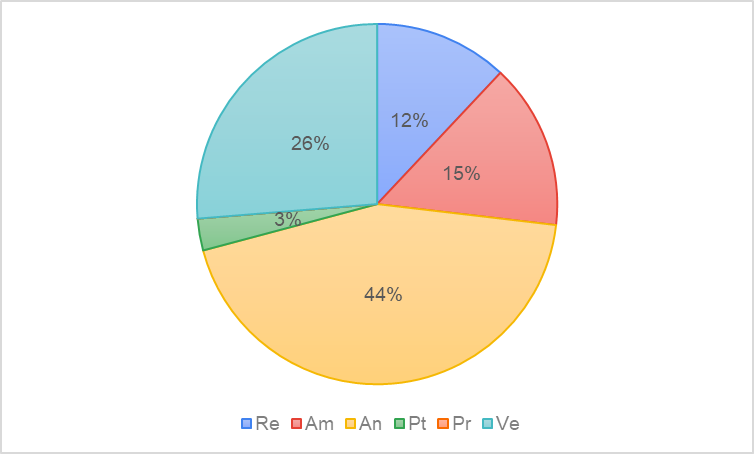
\includegraphics[width=100mm]{./img/Grafici/2.png}
			\caption{Grafico del prospetto economico del periodo di analisi}
		\end{figure}
\subsection{Periodo di progettazione architetturale}
	\subsubsection{Prospetto orario}
	Nel periodo di progettazione\glosp architetturale è prevista la seguente divisione oraria:
	\begin{longtable} {				
		>{}p{40mm}  
		>{}p{8mm}
		>{}p{8mm}
		>{}p{8mm}
		>{}p{8mm}
		>{}p{8mm}
		>{}p{8mm}
		>{}p{12mm}				
	}			
	\rowcolor{gray!50}
	\textbf{Nominativo} & \textbf{Re} & \textbf{Am} & \textbf{An} & \textbf{Pt} & \textbf{Pr} & \textbf{Ve} & \textbf{Totale}	\TBstrut \\ [2mm]
	Corrizzato Vittorio & - & - & 6 & 10 & 5 & 7 & 28 \TBstrut \\ [2mm]
	Dalla Libera Marco & - & 5 & 7 & - & 7 & 9 & 28 \TBstrut \\ [2mm]
	Rampazzo Marco & 6 & - & - & 9 & 8 & 5 & 28 \TBstrut \\ [2mm]
	Santagiuliana Vittorio & - & - & - & 14 & 5 & 9 & 28 \TBstrut \\ [2mm]
	Schiavon Rebecca & 7 & - & - & - & 9 & 12 & 28 \TBstrut \\ [2mm]
	Spreafico Alessandro & - & 5 & 5 & - & 10 & 8 & 28 \TBstrut \\ [2mm]
	Toffoletto Massimo & - & - & 6 & 5 & 7 & 10 & 28 \TBstrut \\ [2mm]
	\rowcolor{white}
	\caption{Prospetto orario del periodo di progettazione\glosp architetturale}
	\end{longtable}
	\pagebreak
	Rappresentata nel seguente grafico:
	\begin{figure} [H]
		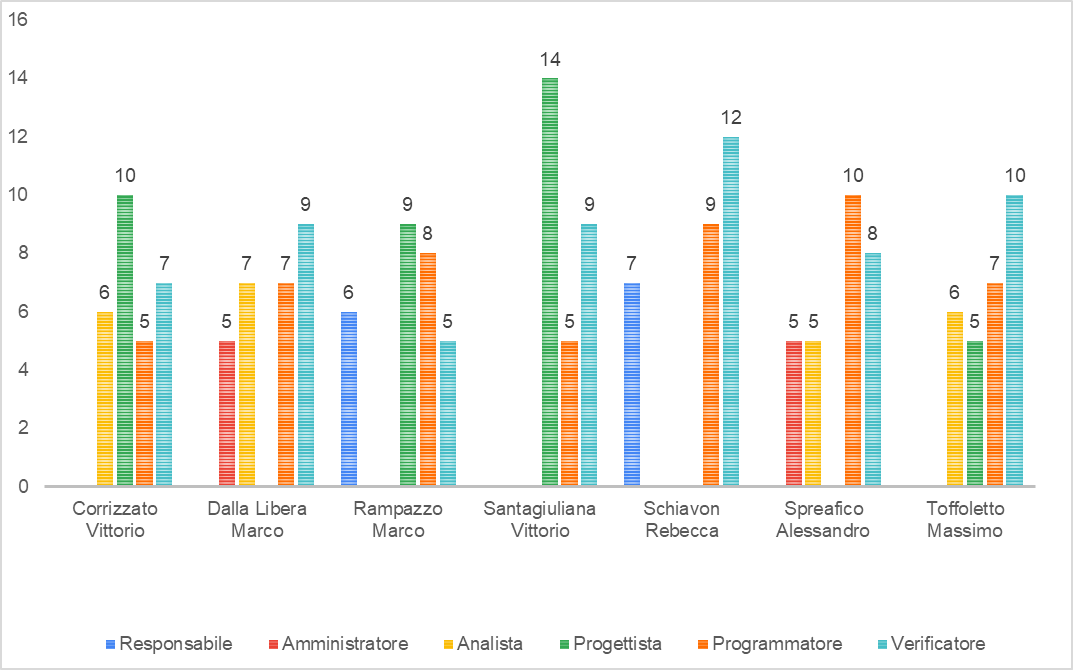
\includegraphics[width=\linewidth]{./img/Grafici/3.png}
		\caption{Grafico del prospetto orario del periodo di progettazione\glosp architetturale}
	\end{figure}

\subsubsection{Prospetto economico}
Nel periodo di progettazione\glosp architetturale sono previsti i seguenti costi:
\begin{longtable} {
		>{}p{32mm}
		>{}p{20mm}
		>{}p{20mm}
	}
	\rowcolor{gray!50}
	
	\textbf{Ruolo} & \textbf{Ore} & \textbf{Costo} \TBstrut \\
	Responsabile & 13 & 390,00\euro{} \TBstrut \\
	Amministratore & 10 & 200,00\euro{} \TBstrut \\
	Analista & 24 & 600,00\euro{} \TBstrut \\
	Progettista & 38 & 836,00\euro{} \TBstrut \\
	Programmatore & 51 & 765,00\euro{} \TBstrut \\
	Verificatore & 60 & 900,00\euro{} \TBstrut \\
	\textbf{Totale} & \textbf{196}& \textbf{3691,00\euro{}} \TBstrut \\	
	\rowcolor{white}
	\caption{Prospetto economico del periodo di progettazione architetturale}
\end{longtable}
\pagebreak
Rappresentati nel seguente grafico:
\begin{figure}[H] 
	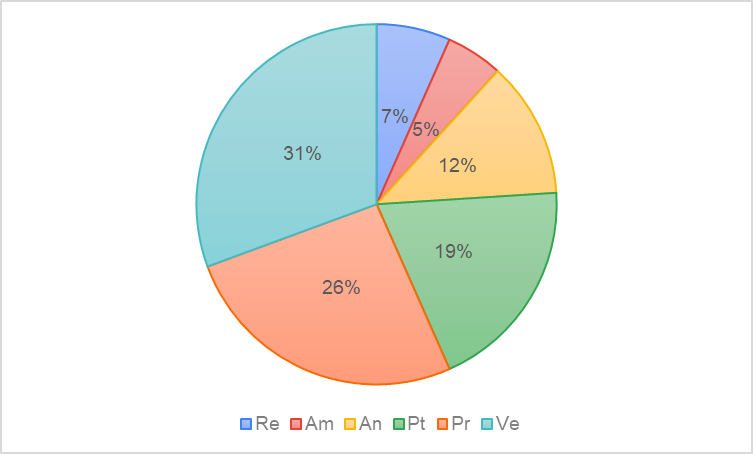
\includegraphics[width=\linewidth]{./img/Grafici/4.png}
	\caption{Grafico del prospetto economico del periodo di progettazione\glosp architetturale}
\end{figure}
\pagebreak
\subsection{Periodo di progettazione dettaglio e codifica}
\subsubsection{Prospetto orario}
Nel periodo di progettazione\glosp dettaglio e codifica è prevista la seguente divisione oraria:
\begin{longtable} {				
		>{}p{40mm}  
		>{}p{8mm}
		>{}p{8mm}
		>{}p{8mm}
		>{}p{8mm}
		>{}p{8mm}
		>{}p{8mm}
		>{}p{12mm}				
	}			
	\rowcolor{gray!50}
	\textbf{Nominativo} & \textbf{Re} & \textbf{Am} & \textbf{An} & \textbf{Pt} & \textbf{Pr} & \textbf{Ve} & \textbf{Totale}	\TBstrut \\ [2mm]
	Corrizzato Vittorio & - & - & 9 & 23 & 22 & - & 54 \TBstrut \\ [2mm]
	Dalla Libera Marco & 9 & - & 6 & 15 & 15 & 9 & 54 \TBstrut \\ [2mm]
	Rampazzo Marco & - & 5 & - & 23 & 18 & 8 & 54 \TBstrut \\ [2mm]
	Santagiuliana Vittorio & 8 & - & - & 20 & 15 & 11 & 54 \TBstrut \\ [2mm]
	Schiavon Rebecca & - & - & 8 & 20 & 18 & 8 & 54 \TBstrut \\ [2mm]
	Spreafico Alessandro & 8 & - & - & 16 & 18 & 12 & 54 \TBstrut \\ [2mm]
	Toffoletto Massimo & - & 5 & - & 23 & 15 & 11 & 54 \TBstrut \\ [2mm]
	\rowcolor{white}
	\caption{Prospetto orario del periodo di progettazione\glosp dettaglio e codifica}
\end{longtable}
\pagebreak
Rappresentata nel seguente grafico:
\begin{figure} [H]
	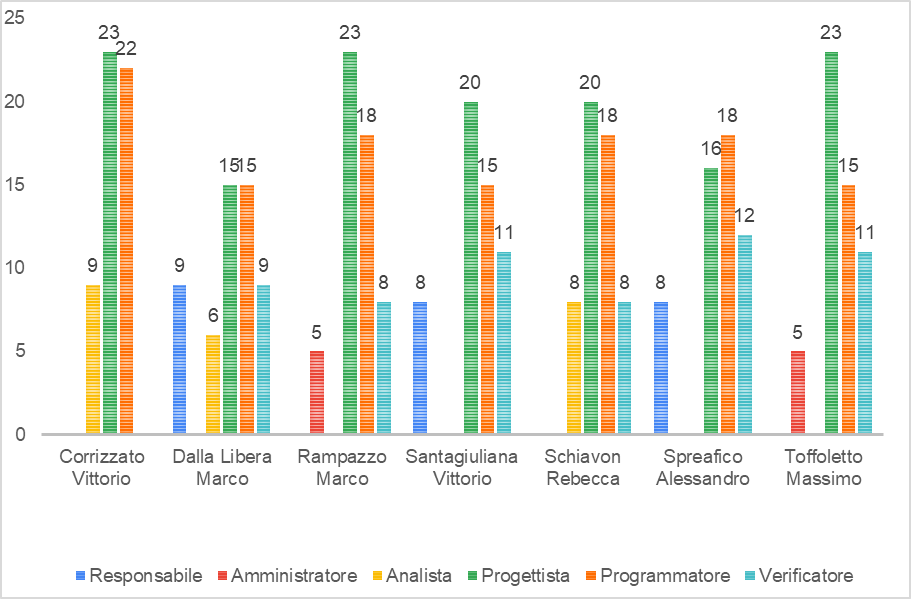
\includegraphics[width=\linewidth]{./img/Grafici/5.png}
	\caption{Grafico del prospetto orario del periodo di progettazione\glosp dettaglio e codifica}
\end{figure}
\mbox{}
In seguito viene presentato il prospetto orario per ogni incremento sviluppato nel macro periodo della progettazione\glosp di dettaglio e codifica. Esso presenta meno ore totali rispetto al prospetto orario precedentemente indicato perché abbiamo rivisto la pianificazione in seguito al consuntivo del periodo precedente. Questa differenza viene discussa nel consuntivo di periodo della progettazione\glosp di dettaglio e codifica.
\paragraph{Incremento 3} \mbox{} \\
Per l'incremento 3 è prevista la seguente divisione oraria:
\begin{longtable} {				
		>{}p{40mm}  
		>{}p{8mm}
		>{}p{8mm}
		>{}p{8mm}
		>{}p{8mm}
		>{}p{8mm}
		>{}p{8mm}
		>{}p{12mm}				
	}			
	\rowcolor{gray!50}
	\textbf{Nominativo} & \textbf{Re} & \textbf{Am} & \textbf{An} & \textbf{Pt} & \textbf{Pr} & \textbf{Ve} & \textbf{Totale}	\TBstrut \\ [2mm]
	Corrizzato Vittorio & - & - & 7 & - & 9 & - & 16 \TBstrut \\ [2mm]
	Dalla Libera Marco & - & - & 3 & - & 14 & - & 17 \TBstrut \\ [2mm]
	Rampazzo Marco & - & 2 & - & 15 & - & - & 17 \TBstrut \\ [2mm]
	Santagiuliana Vittorio & 5 & - & - & 5 & 2 & 5 & 17 \TBstrut \\ [2mm]
	Schiavon Rebecca & - & - & - & 10 & - & 6 & 16 \TBstrut \\ [2mm]
	Spreafico Alessandro & - & - & - & 5 & 7 & 5 & 17 \TBstrut \\ [2mm]
	Toffoletto Massimo & - & - & - & 15 & - & 2 & 17 \TBstrut \\ [2mm]
	\rowcolor{white}
	\caption{Prospetto orario dell'incremento 3}
\end{longtable}
Rappresentata nel seguente grafico:
\begin{figure} [H]
	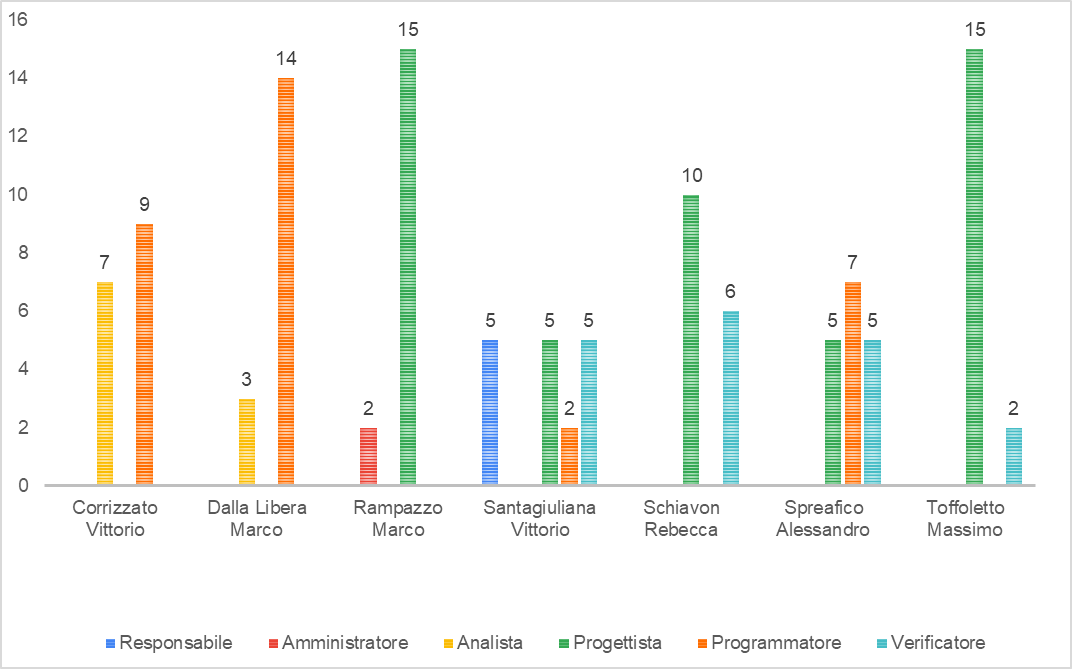
\includegraphics[width=\linewidth]{./img/Grafici/17.png}
	\caption{Grafico del prospetto orario dell'incremento 3}
\end{figure}
\paragraph{Incremento IV} \mbox{} \\
Per l'incremento 4 è prevista la seguente divisione oraria:
\begin{longtable} {				
		>{}p{40mm}  
		>{}p{8mm}
		>{}p{8mm}
		>{}p{8mm}
		>{}p{8mm}
		>{}p{8mm}
		>{}p{8mm}
		>{}p{12mm}				
	}			
	\rowcolor{gray!50}
	\textbf{Nominativo} & \textbf{Re} & \textbf{Am} & \textbf{An} & \textbf{Pt} & \textbf{Pr} & \textbf{Ve} & \textbf{Totale}	\TBstrut \\ [2mm]
	Corrizzato Vittorio & - & - & 1 & 11 & - & - & 12 \TBstrut \\ [2mm]
	Dalla Libera Marco & 4 & - & 1 & 7 & - & - & 12 \TBstrut \\ [2mm]
	Rampazzo Marco & - & - & - & - & 11 & - & 11 \TBstrut \\ [2mm]
	Santagiuliana Vittorio & - & - & - & 2 & 5 & 5 & 12 \TBstrut \\ [2mm]
	Schiavon Rebecca & - & - & 7 & - & 5 & - & 12 \TBstrut \\ [2mm]
	Spreafico Alessandro & - & - & - & - & 5 & 7 & 12 \TBstrut \\ [2mm]
	Toffoletto Massimo & - & 1 & - & - & 6 & 5 & 12 \TBstrut \\ [2mm]
	\rowcolor{white}
	\caption{Prospetto orario dell'incremento 4}
\end{longtable}
Rappresentata nel seguente grafico: \mbox{}
\begin{figure} [H]
	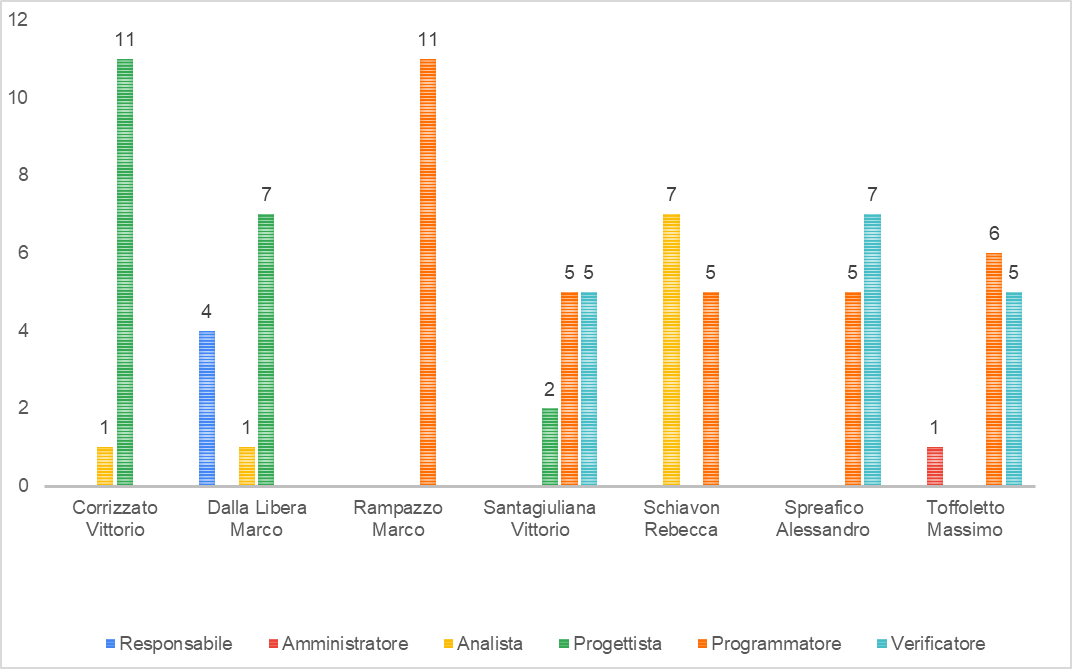
\includegraphics[width=\linewidth]{./img/Grafici/18.png}
	\caption{Grafico del prospetto orario dell'incremento 4}
\end{figure}
\paragraph{Incremento 6} \mbox{} \\
Per l'incremento 6 è prevista la seguente divisione oraria:
\begin{longtable} {				
		>{}p{40mm}  
		>{}p{8mm}
		>{}p{8mm}
		>{}p{8mm}
		>{}p{8mm}
		>{}p{8mm}
		>{}p{8mm}
		>{}p{12mm}				
	}			
	\rowcolor{gray!50}
	\textbf{Nominativo} & \textbf{Re} & \textbf{Am} & \textbf{An} & \textbf{Pt} & \textbf{Pr} & \textbf{Ve} & \textbf{Totale}	\TBstrut \\ [2mm]
	Corrizzato Vittorio & - & - & - & - & 6 & - & 6 \TBstrut \\ [2mm]
	Dalla Libera Marco & - & - & - & 3 & 1 & 1 & 5 \TBstrut \\ [2mm]
	Rampazzo Marco & - & 2 & - & 3 & - & - & 5 \TBstrut \\ [2mm]
	Santagiuliana Vittorio & - & - & - & 5 & - & 1 & 6 \TBstrut \\ [2mm]
	Schiavon Rebecca & - & - & - & 4 & - & 2 & 6 \TBstrut \\ [2mm]
	Spreafico Alessandro & 4 & - & - & 2 & - & - & 6 \TBstrut \\ [2mm]
	Toffoletto Massimo & - & - & - & 3 & 3 & - & 6 \TBstrut \\ [2mm]
	\rowcolor{white}
	\caption{Prospetto orario dell'incremento VI}
\end{longtable}
Rappresentata nel seguente grafico:
\begin{figure} [H]
	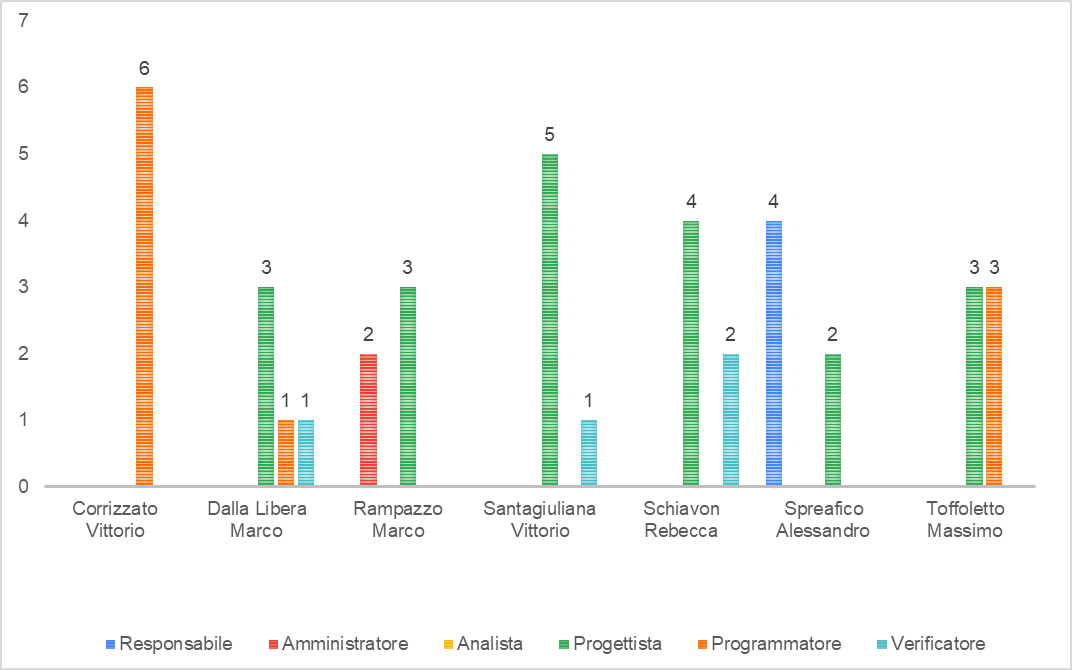
\includegraphics[width=\linewidth]{./img/Grafici/19.png}
	\caption{Grafico del prospetto orario dell'incremento 6}
\end{figure}
\paragraph{Incremento 13} \mbox{} \\
Per l'incremento 13 è prevista la seguente divisione oraria:
\begin{longtable} {				
		>{}p{40mm}  
		>{}p{8mm}
		>{}p{8mm}
		>{}p{8mm}
		>{}p{8mm}
		>{}p{8mm}
		>{}p{8mm}
		>{}p{12mm}				
	}			
	\rowcolor{gray!50}
	\textbf{Nominativo} & \textbf{Re} & \textbf{Am} & \textbf{An} & \textbf{Pt} & \textbf{Pr} & \textbf{Ve} & \textbf{Totale}	\TBstrut \\ [2mm]
	Corrizzato Vittorio & - & - & - & 4 & - & - & 4 \TBstrut \\ [2mm]
	Dalla Libera Marco & 4 & - & - & - & - & - & 4 \TBstrut \\ [2mm]
	Rampazzo Marco & - & 1 & - & - & 3 & - & 4 \TBstrut \\ [2mm]
	Santagiuliana Vittorio & - & - & - & - & 3 & - & 3 \TBstrut \\ [2mm]
	Schiavon Rebecca & - & - & - & 2 & 2 & - & 4 \TBstrut \\ [2mm]
	Spreafico Alessandro & - & - & - & 4 & - & - & 4 \TBstrut \\ [2mm]
	Toffoletto Massimo & - & 1 & - & - & - & 3 & 4 \TBstrut \\ [2mm]
	\rowcolor{white}
	\caption{Prospetto orario dell'incremento 13}
\end{longtable}
Rappresentata nel seguente grafico:
\begin{figure} [H]
	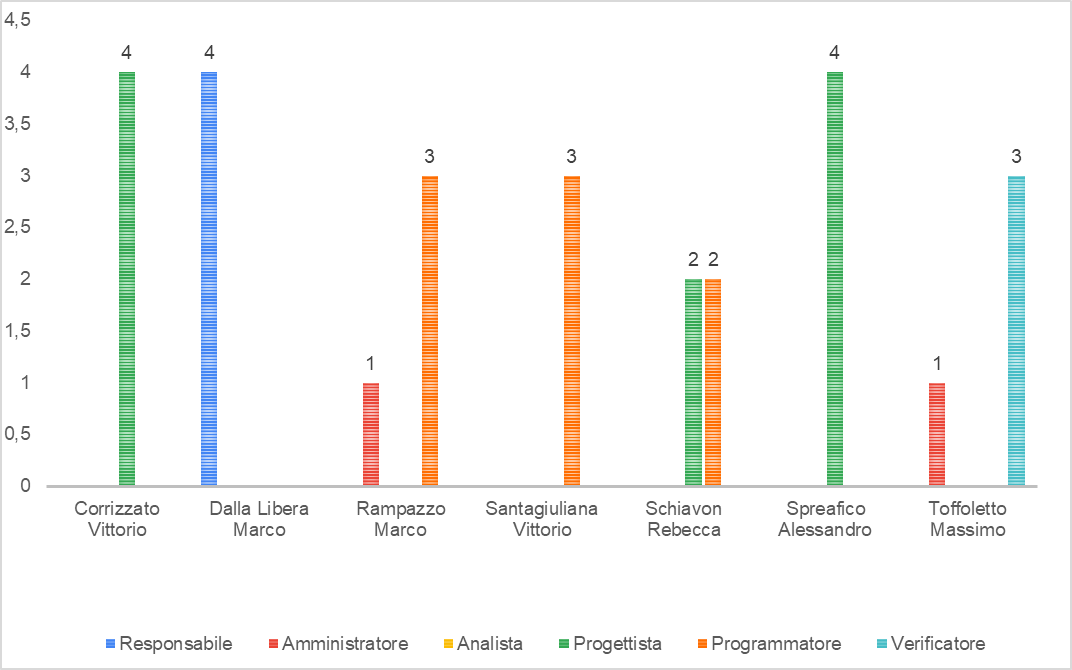
\includegraphics[width=\linewidth]{./img/Grafici/20.png}
	\caption{Grafico del prospetto orario dell'incremento 13}
\end{figure}
\paragraph{Incremento 14} \mbox{} \\
Per l'incremento 14 è prevista la seguente divisione oraria:
\begin{longtable} {				
		>{}p{40mm}  
		>{}p{8mm}
		>{}p{8mm}
		>{}p{8mm}
		>{}p{8mm}
		>{}p{8mm}
		>{}p{8mm}
		>{}p{12mm}				
	}			
	\rowcolor{gray!50}
	\textbf{Nominativo} & \textbf{Re} & \textbf{Am} & \textbf{An} & \textbf{Pt} & \textbf{Pr} & \textbf{Ve} & \textbf{Totale}	\TBstrut \\ [2mm]
	Corrizzato Vittorio & - & - & - & 4 & 7 & - & 11 \TBstrut \\ [2mm]
	Dalla Libera Marco & - & - & - & 4 & - & 8 & 12 \TBstrut \\ [2mm]
	Rampazzo Marco & - & - & - & 5 & 2 & 5 & 12 \TBstrut \\ [2mm]
	Santagiuliana Vittorio & - & - & - & 8 & 4 & - & 12 \TBstrut \\ [2mm]
	Schiavon Rebecca & - & - & - & 2 & 10 & - & 12 \TBstrut \\ [2mm]
	Spreafico Alessandro & 4 & - & - & 4 & 2 & - & 10 \TBstrut \\ [2mm]
	Toffoletto Massimo & - & 2 & - & 3 & 3 & 1 & 9 \TBstrut \\ [2mm]
	\rowcolor{white}
	\caption{Prospetto orario dell'incremento 14}
\end{longtable}
Rappresentata nel seguente grafico:
\begin{figure} [H]
	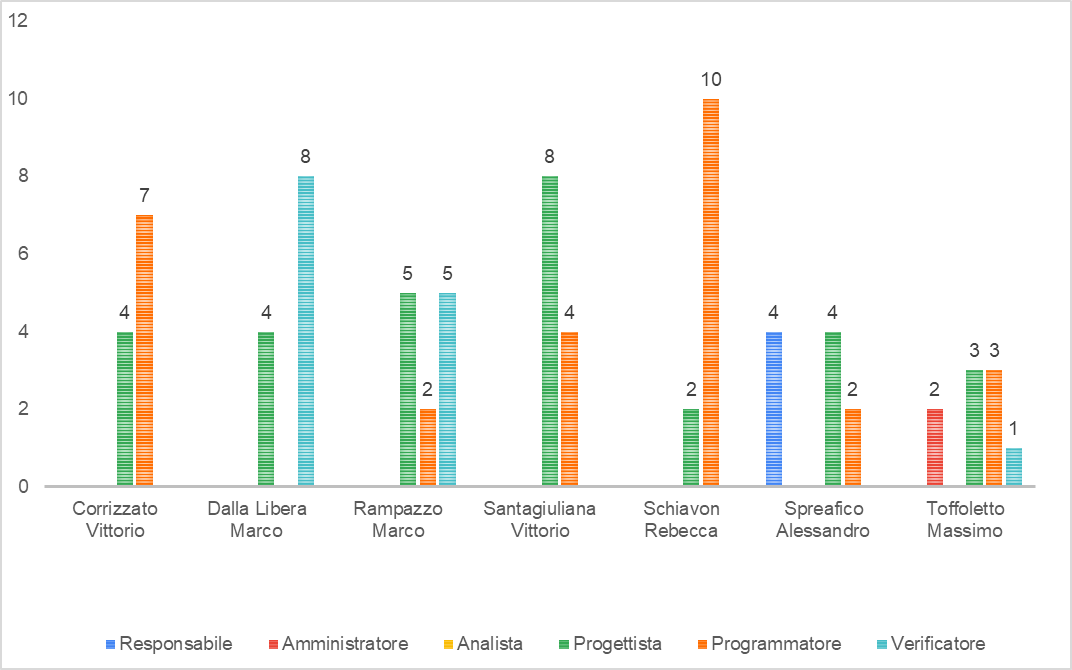
\includegraphics[width=\linewidth]{./img/Grafici/21.png}
	\caption{Grafico del prospetto orario dell'incremento 14}
\end{figure}
\paragraph{Incremento 16} \mbox{} \\
Per l'incremento 16 è prevista la seguente divisione oraria:
\begin{longtable} {				
		>{}p{40mm}  
		>{}p{8mm}
		>{}p{8mm}
		>{}p{8mm}
		>{}p{8mm}
		>{}p{8mm}
		>{}p{8mm}
		>{}p{12mm}				
	}			
	\rowcolor{gray!50}
	\textbf{Nominativo} & \textbf{Re} & \textbf{Am} & \textbf{An} & \textbf{Pt} & \textbf{Pr} & \textbf{Ve} & \textbf{Totale}	\TBstrut \\ [2mm]
	Corrizzato Vittorio & - & - & - & 4 & - & - & 4 \TBstrut \\ [2mm]
	Dalla Libera Marco & 1 & - & - & 2 & - & - & 3 \TBstrut \\ [2mm]
	Rampazzo Marco & - & - & - & 1 & - & 3 & 4 \TBstrut \\ [2mm]
	Santagiuliana Vittorio & 3 & - & - & - & - & - & 3 \TBstrut \\ [2mm]
	Schiavon Rebecca & - & - & - & 2 & 1 & - & 3 \TBstrut \\ [2mm]
	Spreafico Alessandro & - & - & - & - & 4 & - & 4 \TBstrut \\ [2mm]
	Toffoletto Massimo & - & 1 & - & 1 & 3 & - & 5 \TBstrut \\ [2mm]
	\rowcolor{white}
	\caption{Prospetto orario dell'incremento 16}
\end{longtable}
Rappresentata nel seguente grafico:
\begin{figure} [H]
	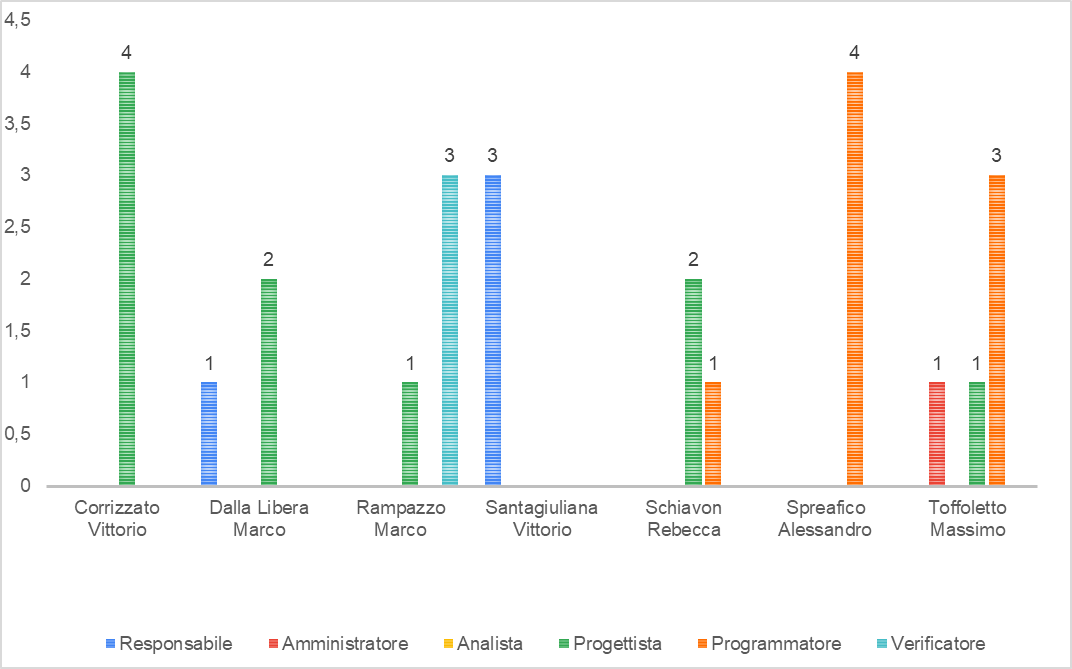
\includegraphics[width=\linewidth]{./img/Grafici/22.png}
	\caption{Grafico del prospetto orario dell'incremento 16}
\end{figure}
\subsubsection{Prospetto economico}
Nel periodo di progettazione\glosp dettaglio e codifica sono previsti i seguenti costi:
\begin{longtable} {
		>{}p{32mm}
		>{}p{20mm}
		>{}p{20mm}
	}
	\rowcolor{gray!50}
	
	\textbf{Ruolo} & \textbf{Ore} & \textbf{Costo} \TBstrut \\
	Responsabile & 25 & 750,00\euro{} \TBstrut \\
	Amministratore & 10 & 200,00\euro{} \TBstrut \\
	Analista & 23 & 575,00\euro{} \TBstrut \\
	Progettista & 140 & 3080,00\euro{}\TBstrut \\
	Programmatore & 121 & 1815,00\euro{} \TBstrut \\
	Verificatore & 59 & 885,00\euro{} \TBstrut \\
	\textbf{Totale} & \textbf{378}& \textbf{7305,00\euro{}} \TBstrut \\	
	\rowcolor{white}
	\caption{Prospetto economico del periodo di progettazione\glosp dettaglio e codifica}
\end{longtable} \mbox{} \\
Rappresentati nel seguente grafico: \mbox{}
\begin{figure} [h!]
	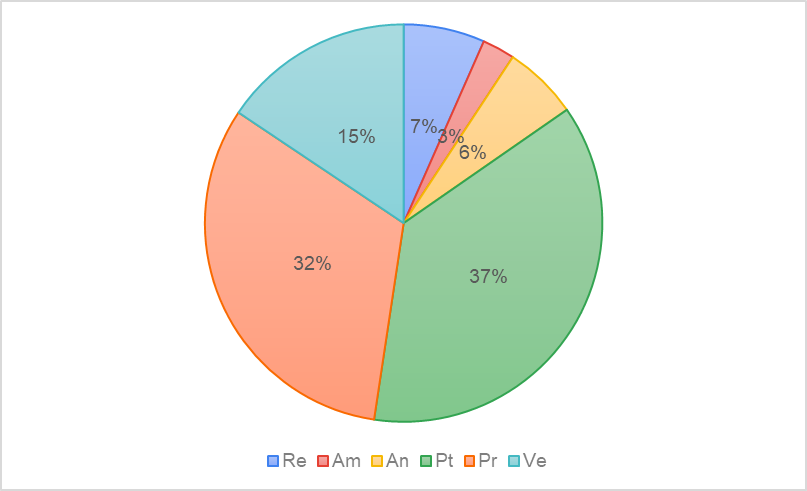
\includegraphics[width=\linewidth]{./img/Grafici/6.png}
	\caption{Grafico del prospetto economico del periodo di progettazione\glosp dettaglio e codifica}
\end{figure}
\mbox{} \\
In seguito viene presentato il prospetto economico per ogni incremento sviluppato nel macro periodo della progettazione\glosp di dettaglio e codifica. Presenta un costo totale minore rispetto al prospetto orario precedentemente indicato perché abbiamo rivisto la pianificazione in seguito al consuntivo del periodo precedente. Questa differenza viene discussa nel consuntivo di periodo della progettazione\glosp di dettaglio e codifica.
\paragraph{Incremento 3} \mbox{} \\
Per l'incremento 3 sono previsti i seguenti costi:
\begin{longtable} {
		>{}p{32mm}
		>{}p{20mm}
		>{}p{20mm}
	}
	\rowcolor{gray!50}
	
	\textbf{Ruolo} & \textbf{Ore} & \textbf{Costo} \TBstrut \\
	Responsabile & 5 & 150,00\euro{} \TBstrut \\
	Amministratore & 2 & 40,00\euro{} \TBstrut \\
	Analista & 10 & 250,00\euro{} \TBstrut \\
	Progettista & 50 & 1100,00\euro{}\TBstrut \\
	Programmatore & 32 & 480,00\euro{} \TBstrut \\
	Verificatore & 18 & 270,00\euro{} \TBstrut \\
	\textbf{Totale} & \textbf{117}& \textbf{2290,00\euro{}} \TBstrut \\	
	\rowcolor{white}
	\caption{Prospetto economico dell'incremento 3}
\end{longtable} \mbox{} \\
Rappresentati nel seguente grafico: \mbox{}
\begin{figure} [H]
	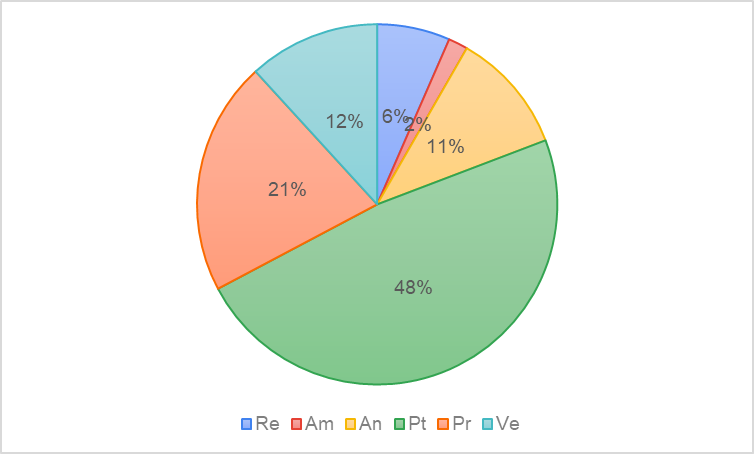
\includegraphics[width=\linewidth]{./img/Grafici/23.png}
	\caption{Grafico del prospetto economico dell'incremento 3}
\end{figure}
\paragraph{Incremento 4} \mbox{} \\
Per l'incremento 4 sono previsti i seguenti costi:
\begin{longtable} {
		>{}p{32mm}
		>{}p{20mm}
		>{}p{20mm}
	}
	\rowcolor{gray!50}
	
	\textbf{Ruolo} & \textbf{Ore} & \textbf{Costo} \TBstrut \\
	Responsabile & 4 & 120,00\euro{} \TBstrut \\
	Amministratore & 1 & 20,00\euro{} \TBstrut \\
	Analista & 9 & 225,00\euro{} \TBstrut \\
	Progettista & 20 & 440,00\euro{}\TBstrut \\
	Programmatore & 32 & 480,00\euro{} \TBstrut \\
	Verificatore & 17 & 255,00\euro{} \TBstrut \\
	\textbf{Totale} & \textbf{83}& \textbf{1540,00\euro{}} \TBstrut \\	
	\rowcolor{white}
	\caption{Prospetto economico dell'incremento 4}
\end{longtable} \mbox{} \\
Rappresentati nel seguente grafico: \mbox{}
\begin{figure} [H]
	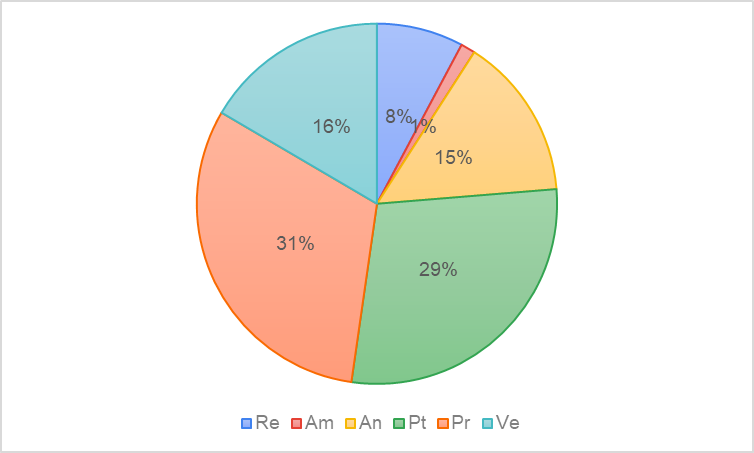
\includegraphics[width=\linewidth]{./img/Grafici/24.png}
	\caption{Grafico del prospetto economico dell'incremento 4}
\end{figure}
\paragraph{Incremento 6} \mbox{} \\
Per l'incremento 6 sono previsti i seguenti costi:
\begin{longtable} {
		>{}p{32mm}
		>{}p{20mm}
		>{}p{20mm}
	}
	\rowcolor{gray!50}
	
	\textbf{Ruolo} & \textbf{Ore} & \textbf{Costo} \TBstrut \\
	Responsabile & 4 & 120,00\euro{} \TBstrut \\
	Amministratore & 2 & 40,00\euro{} \TBstrut \\
	Analista & - & - \TBstrut \\
	Progettista & 20 & 440,00\euro{}\TBstrut \\
	Programmatore & 10 & 150,00\euro{} \TBstrut \\
	Verificatore & 4 & 60,00\euro{} \TBstrut \\
	\textbf{Totale} & \textbf{40}& \textbf{810,00\euro{}} \TBstrut \\	
	\rowcolor{white}
	\caption{Prospetto economico dell'incremento 6}
\end{longtable} \mbox{} \\
Rappresentati nel seguente grafico: \mbox{}
\begin{figure} [H]
	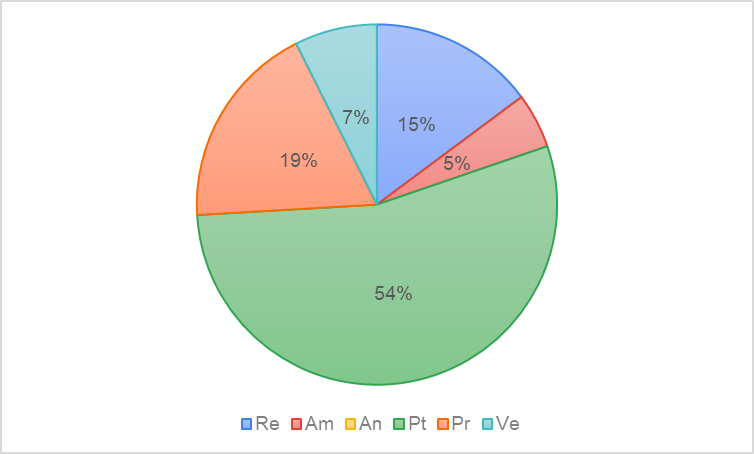
\includegraphics[width=\linewidth]{./img/Grafici/25.png}
	\caption{Grafico del prospetto economico dell'incremento 6}
\end{figure}
\paragraph{Incremento 13} \mbox{} \\
Per l'incremento 13 sono previsti i seguenti costi:
\begin{longtable} {
		>{}p{32mm}
		>{}p{20mm}
		>{}p{20mm}
	}
	\rowcolor{gray!50}
	
	\textbf{Ruolo} & \textbf{Ore} & \textbf{Costo} \TBstrut \\
	Responsabile & 4 & 120,00\euro{} \TBstrut \\
	Amministratore & 2 & 40,00\euro{} \TBstrut \\
	Analista & - & - \TBstrut \\
	Progettista & 10 & 220,00\euro{}\TBstrut \\
	Programmatore & 8 & 120,00\euro{} \TBstrut \\
	Verificatore & 3 & 45,00\euro{} \TBstrut \\
	\textbf{Totale} & \textbf{27}& \textbf{545,00\euro{}} \TBstrut \\	
	\rowcolor{white}
	\caption{Prospetto economico dell'incremento 13}
\end{longtable} \mbox{} \\
Rappresentati nel seguente grafico: 
\begin{figure} [h!]
	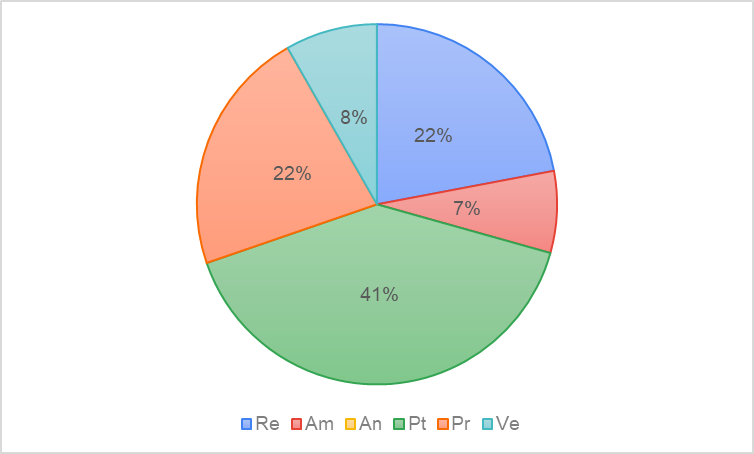
\includegraphics[width=\linewidth]{./img/Grafici/26.png}
	\caption{Grafico del prospetto economico dell'incremento 13}
\end{figure}
\paragraph{Incremento 14} \mbox{} \\
Per l'incremento 14 sono previsti i seguenti costi:
\begin{longtable} {
		>{}p{32mm}
		>{}p{20mm}
		>{}p{20mm}
	}
	\rowcolor{gray!50}
	
	\textbf{Ruolo} & \textbf{Ore} & \textbf{Costo} \TBstrut \\
	Responsabile & 4 & 120,00\euro{} \TBstrut \\
	Amministratore & 2 & 40,00\euro{} \TBstrut \\
	Analista & - & - \TBstrut \\
	Progettista & 30 & 660,00\euro{}\TBstrut \\
	Programmatore & 28 & 420,00\euro{} \TBstrut \\
	Verificatore & 14 & 210,00\euro{} \TBstrut \\
	\textbf{Totale} & \textbf{78}& \textbf{1450,00\euro{}} \TBstrut \\	
	\rowcolor{white}
	\caption{Prospetto economico dell'incremento 14}
\end{longtable} \mbox{} \\
Rappresentati nel seguente grafico: \mbox{}
\begin{figure} [H]
	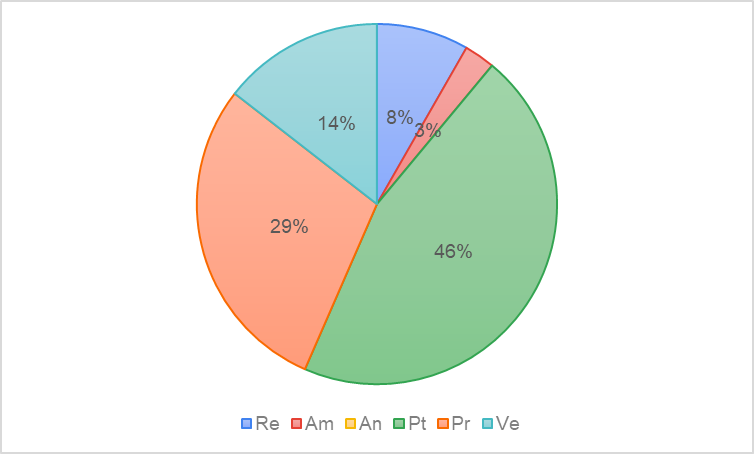
\includegraphics[width=\linewidth]{./img/Grafici/27.png}
	\caption{Grafico del prospetto economico dell'incremento 14}
\end{figure}
\paragraph{Incremento 16} \mbox{} \\
Per l'incremento 16 sono previsti i seguenti costi:
\begin{longtable} {
		>{}p{32mm}
		>{}p{20mm}
		>{}p{20mm}
	}
	\rowcolor{gray!50}
	
	\textbf{Ruolo} & \textbf{Ore} & \textbf{Costo} \TBstrut \\
	Responsabile & 4 & 120,00\euro{} \TBstrut \\
	Amministratore & 1 & 20,00\euro{} \TBstrut \\
	Analista & - & - \TBstrut \\
	Progettista & 10 & 220,00\euro{}\TBstrut \\
	Programmatore & 8 & 120,00\euro{} \TBstrut \\
	Verificatore & 3 & 45,00\euro{} \TBstrut \\
	\textbf{Totale} & \textbf{26}& \textbf{525,00\euro{}} \TBstrut \\	
	\rowcolor{white}
	\caption{Prospetto economico dell'incremento 16}
\end{longtable} \mbox{} \\
Rappresentati nel seguente grafico: \mbox{}
\begin{figure} [H]
	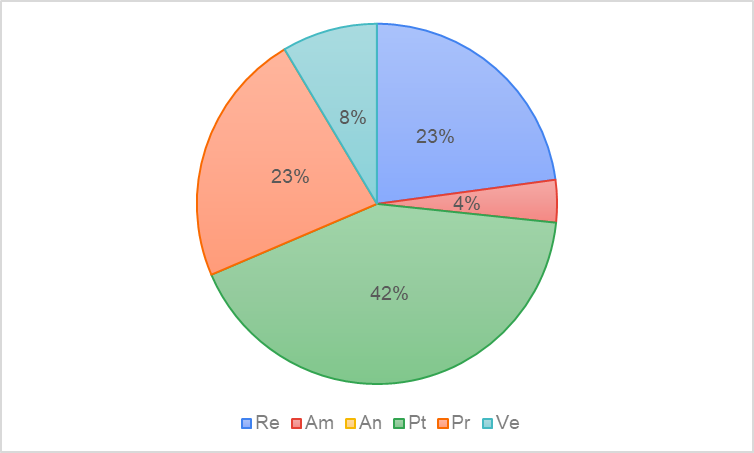
\includegraphics[width=\linewidth]{./img/Grafici/28.png}
	\caption{Grafico del prospetto economico dell'incremento 16}
\end{figure}
\subsection{Periodo di validazione e collaudo}
\subsubsection{Prospetto orario}
Nel periodo di validazione\glosp e collaudo è prevista la seguente divisione oraria:
\begin{longtable} {				
		>{}p{40mm}  
		>{}p{8mm}
		>{}p{8mm}
		>{}p{8mm}
		>{}p{8mm}
		>{}p{8mm}
		>{}p{8mm}
		>{}p{12mm}			
	}			
	\rowcolor{gray!50}
	\textbf{Nominativo} & \textbf{Re} & \textbf{Am} & \textbf{An} & \textbf{Pt} & \textbf{Pr} & \textbf{Ve} & \textbf{Totale}	\TBstrut \\ [2mm]
	Corrizzato Vittorio & - & - & - & - & 10 & 10 & 20 \TBstrut \\ [2mm]
	Dalla Libera Marco & 8 & 5 & - & - & 7 & - & 20 \TBstrut \\ [2mm]
	Rampazzo Marco & - & - & - & 5 & 8 & 7 & 20 \TBstrut \\ [2mm]
	Santagiuliana Vittorio & - & 5 & - & - & 6 & 9 & 20 \TBstrut \\ [2mm]
	Schiavon Rebecca & - & 8 & - & - & 7 & 5 & 20 \TBstrut \\ [2mm]
	Spreafico Alessandro & - & - & - & - & 8 & 12 & 20 \TBstrut \\ [2mm]
	Toffoletto Massimo & - & - & - & - & 9 & 11 & 20 \TBstrut \\ [2mm]
	\rowcolor{white}
	\caption{Prospetto orario del periodo di validazione\glosp e collaudo}
\end{longtable}
Rappresentata nel seguente grafico:
\begin{figure} [H]
	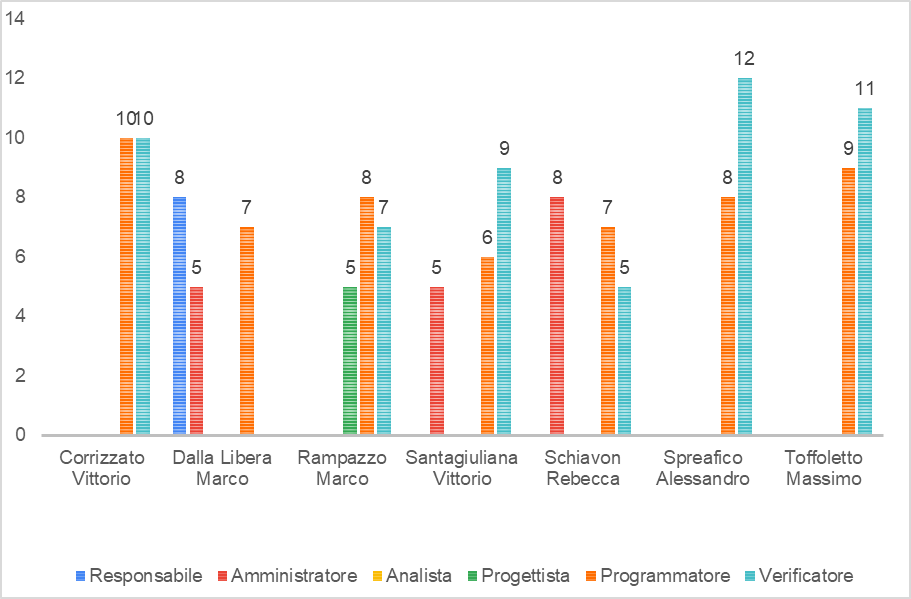
\includegraphics[width=\linewidth]{./img/Grafici/7.png}
	\caption{Grafico del prospetto orario del periodo di validazione\glosp e collaudo}
\end{figure}
\pagebreak
\subsubsection{Prospetto economico}
Nel periodo di validazione\glosp e collaudo sono previsti i seguenti costi:
\begin{longtable} {
		>{}p{32mm}
		>{}p{20mm}
		>{}p{20mm}
	}
	\rowcolor{gray!50}
	
	\textbf{Ruolo} & \textbf{Ore} & \textbf{Costo} \TBstrut \\
	Responsabile & 8 & 240,00\euro{} \TBstrut \\
	Amministratore & 18 & 360,00\euro{} \TBstrut \\
	Analista & 0 & 0,00\euro{} \TBstrut \\
	Progettista & 5 & 110,00\euro{} \TBstrut \\
	Programmatore & 55 & 825,00\euro{} \TBstrut \\
	Verificatore & 54 & 810,00\euro{} \TBstrut \\
	\textbf{Totale} & \textbf{140}& \textbf{2345,00\euro{}} \TBstrut \\	
	\rowcolor{white}
	\caption{Prospetto economico del periodo di validazione\glosp e collaudo}
\end{longtable}
Rappresentati nel seguente grafico:
\begin{figure} [H]
	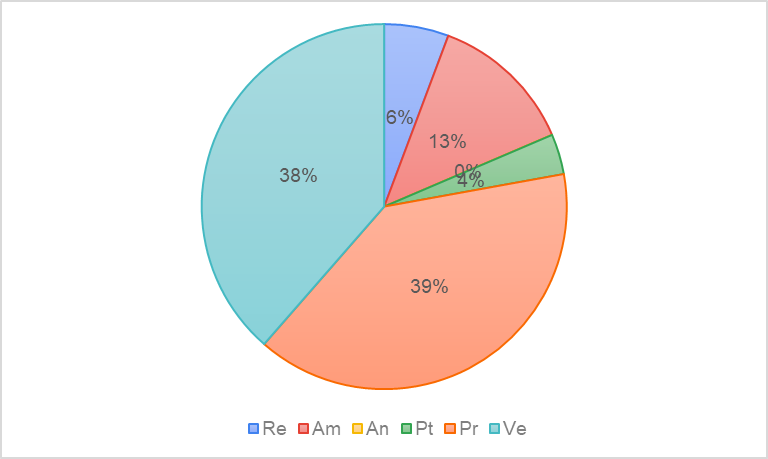
\includegraphics[width=\linewidth]{./img/Grafici/8.png}
	\caption{Grafico del prospetto economico del periodo di validazione \glosp e collaudo}
\end{figure}

\subsection{Totale ore investite}
\subsubsection{Prospetto orario}
La seguente tabella presenta la suddivisione delle ore investite per l'intero progetto\glo:
\begin{longtable} {				
		>{}p{40mm}  
		>{}p{8mm}
		>{}p{8mm}
		>{}p{8mm}
		>{}p{8mm}
		>{}p{8mm}
		>{}p{8mm}
		>{}p{12mm}			
	}			
	\rowcolor{gray!50}
	\textbf{Nominativo} & \textbf{Re} & \textbf{Am} & \textbf{An} & \textbf{Pt} & \textbf{Pr} & \textbf{Ve} & \textbf{Totale}	\TBstrut \\ [2mm]
	Corrizzato Vittorio & 6 & 6 & 23 & 33 & 37 & 22 & 127 \TBstrut \\ [2mm]
	Dalla Libera Marco & 24 & 10 & 26 & 15 & 29 & 23 & 127 \TBstrut \\ [2mm]
	Rampazzo Marco & 6 & 13 & 12 & 37 & 34 & 25 & 127 \TBstrut \\ [2mm]
	Santagiuliana Vittorio & 8 & 10 & 12 & 34 & 26 & 37 & 127 \TBstrut \\ [2mm]
	Schiavon Rebecca & 7 & 8 & 23 & 20 & 34 & 35 & 127 \TBstrut \\ [2mm]
	Spreafico Alessandro & 8 & 5 & 17 & 21 & 36 & 40 & 127 \TBstrut \\ [2mm]
	Toffoletto Massimo & 8 & 12 & 11 & 28 & 31 & 37 & 127 \TBstrut \\ [2mm]
	\rowcolor{white}
	\caption{Prospetto orario del totale di ore investite}
\end{longtable}
\pagebreak
Rappresentata anche nel seguente grafico:
\begin{figure} [H]
	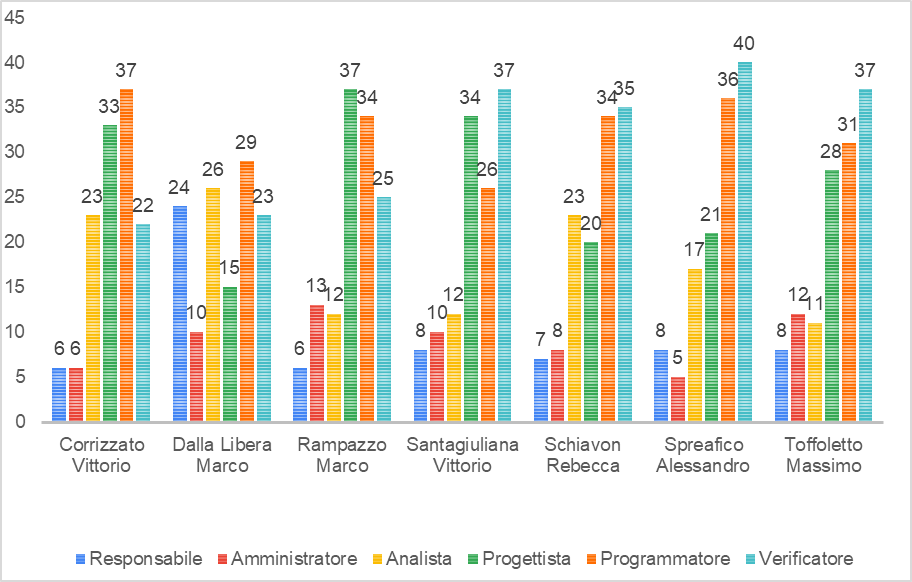
\includegraphics[width=\linewidth]{./img/Grafici/9.png}
	\caption{Grafico del prospetto orario delle ore investite per l'intero progetto\glo}
\end{figure}

\subsubsection{Prospetto economico}
La seguente tabella presenta i costi delle ore investite per l'intero progetto\glo:
\begin{longtable} {
		>{}p{32mm}
		>{}p{20mm}
		>{}p{20mm}
	}
	\rowcolor{gray!50}
	
	\textbf{Ruolo} & \textbf{Ore} & \textbf{Costo} \TBstrut \\
	Responsabile & 67 & 2010,00\euro{} \TBstrut \\
	Amministratore & 64 & 1280,00\euro{} \TBstrut \\
	Analista & 124 & 3100,00\euro{} \TBstrut \\
	Progettista & 188 & 4136,00\euro{} \TBstrut \\
	Programmatore & 227 & 3405,00\euro{} \TBstrut \\
	Verificatore & 219 & 3285,00\euro{} \TBstrut \\
	\textbf{Totale} & \textbf{749}& \textbf{17216,00\euro{}} \TBstrut \\		
	\rowcolor{white}
	\caption{Prospetto economico del totale di ore investite}
\end{longtable} \mbox{} \\ \\ \\
Rappresentati anche nel seguente grafico:
\begin{figure} [H]
	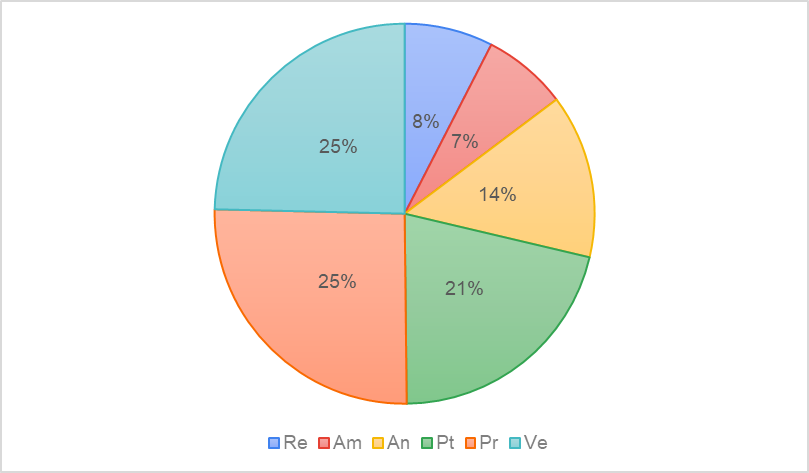
\includegraphics[width=\linewidth]{./img/Grafici/10.png}
	\caption{Grafico del prospetto economico delle ore investite per l'intero progetto\glo}
\end{figure}

\subsection{Totale ore rendicontate}
\subsubsection{Prospetto orario}
La seguente tabella presenta la suddivisione delle ore rendicontate per l'intero progetto\glo:
\begin{longtable} {				
		>{}p{40mm}  
		>{}p{8mm}
		>{}p{8mm}
		>{}p{8mm}
		>{}p{8mm}
		>{}p{8mm}
		>{}p{8mm}
		>{}p{12mm}			
	}			
	\rowcolor{gray!50}
	\textbf{Nominativo} & \textbf{Re} & \textbf{Am} & \textbf{An} & \textbf{Pt} & \textbf{Pr} & \textbf{Ve} & \textbf{Totale}	\TBstrut \\ [2mm]
	Corrizzato Vittorio & - & - & 15 & 33 & 37 & 17 & 102 \TBstrut \\ [2mm]
	Dalla Libera Marco & 17 & 10 & 13 & 15 & 29 & 18 & 102 \TBstrut \\ [2mm]
	Rampazzo Marco & 6 & 5 & - & 37 & 34 & 20 & 102 \TBstrut \\ [2mm]
	Santagiuliana Vittorio & 8 & 5 & - & 34 & 26 & 29 & 102 \TBstrut \\ [2mm]
	Schiavon Rebecca & 7 & 8 & 8 & 20 & 34 & 25 & 102 \TBstrut \\ [2mm]
	Spreafico Alessandro & 8 & 5 & 5 & 16 & 36 & 32 & 102 \TBstrut \\ [2mm]
	Toffoletto Massimo & - & 5 & 6 & 28 & 31 & 32 & 102 \TBstrut \\ [2mm]
	\rowcolor{white}
	\caption{Prospetto orario del totale di ore rendicontate}
\end{longtable}
Rappresentata anche nel seguente grafico:
\begin{figure} [H]
	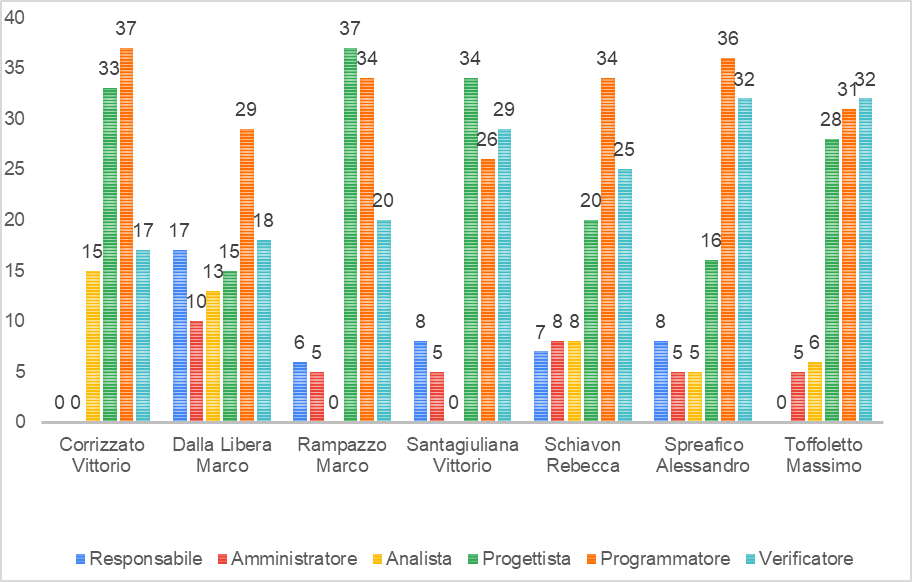
\includegraphics[width=\linewidth]{./img/Grafici/11.png}
	\caption{Grafico del prospetto orario delle ore rendicontate per l'intero progetto\glo}
\end{figure}
\pagebreak
\subsubsection{Prospetto economico}
La seguente tabella presenta i costi delle ore rendicontate per l'intero progetto\glo
\begin{longtable} {
		>{}p{32mm}
		>{}p{20mm}
		>{}p{20mm}
	}
	\rowcolor{gray!50}
	
	\textbf{Ruolo} & \textbf{Ore} & \textbf{Costo} \TBstrut \\
	Responsabile & 46 & 1380,00\euro{} \TBstrut \\
	Amministratore & 38 & 760,00\euro{} \TBstrut \\
	Analista & 47 & 1175,00\euro{} \TBstrut \\
	Progettista & 183 & 4026,00\euro{} \TBstrut \\
	Programmatore & 227 & 3405,00\euro{} \TBstrut \\
	Verificatore & 173 & 2595,00\euro{} \TBstrut \\
	\textbf{Totale} & \textbf{714}& \textbf{13341,00\euro{}} \TBstrut \\		
	\rowcolor{white}
	\caption{Prospetto economico del totale di ore rendicontate}
\end{longtable} \mbox{} \\ \\
Rappresentati anche nel seguente grafico:
\begin{figure} [H]
	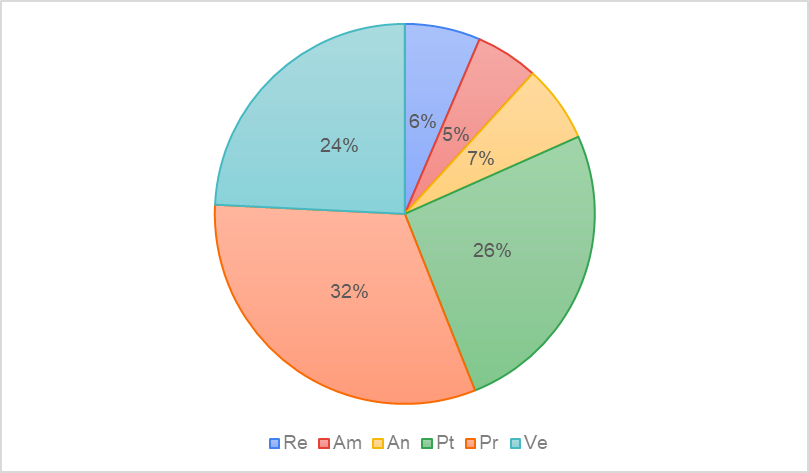
\includegraphics[width=\linewidth]{./img/Grafici/12.png}
	\caption{Grafico del prospetto economico delle ore rendicontate per l'intero progetto\glo}
\end{figure}
	
\section{Consuntivi di periodo}
Vengono riportati gli effettivi costi sostenuti per ogni periodo con le eventuali differenze rispetto a quanto preventivato. Il bilancio risulterà quindi:
\begin{itemize}
	\item \textbf{Positivo}: se i costi del consuntivo risultano minori di quelli del preventivo;
	\item \textbf{Pari}: se i costi del consuntivo risultano uguali a quelli del preventivo;
	\item \textbf{Negativo}: se i costi del consuntivo risultano superiori a quelli del preventivo.
\end{itemize}
Seguiranno quindi le conclusioni con le motivazioni delle eventuali differenze e le contromisure che il gruppo ha deciso di attuare per evitare ulteriori discrepanze con quanto dichiarato nel preventivo.
	\subsection{Periodo di Analisi}
	La tabella riporta il numero di ore effettivamente svolte dal gruppo e il rispettivo costo con le eventuali differenze rilevate rispetto al preventivo
	\begin{longtable} {							
			>{}p{40mm}  
			>{}p{20mm}	
			>{}p{28mm}			
		}			
		\rowcolor{gray!50}
		
		\textbf{Ruolo} & \textbf{Ore} & \textbf{Costo} \TBstrut \\
		Responsabile & 20(-1) & 600\euro{}(-30\euro{}) \TBstrut \\
		Amministratore & 26 & 520\euro{} \TBstrut \\
		Analista & 86(+9)& 2150\euro{}(+225\euro{}) \TBstrut \\
		Progettista & 10(+5) & 220\euro{}(+110\euro{}) \TBstrut \\
		Programmatore & 0 & 0\euro{} \TBstrut \\
		Verificatore & 46 & 690\euro{} \TBstrut \\
		\textbf{Totale Preventivo} & 175 & 3875\euro{}	\TBstrut \\	
		\textbf{Totale Consuntivo} & 188 & 4180\euro{}	\TBstrut \\	
		\textbf{Differenza Totale} & +13 & +305\euro{} \TBstrut \\
		\rowcolor{white}
		\caption{Numero di ore effettivamente svolte con rispettivo costo e differenze rispetto al preventivo}	
	\end{longtable}
	\pagebreak
	Rappresentate anche dai grafici:
	\begin{figure} [H]
		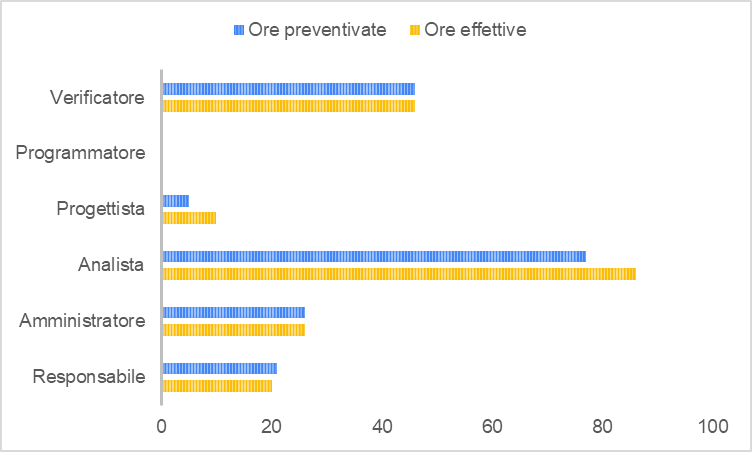
\includegraphics[width=\linewidth]{./img/Grafici/13.png}
		\caption{Grafico delle ore preventivate rispetto alle ore effettive}
	\end{figure}

	\begin{figure} [H]
		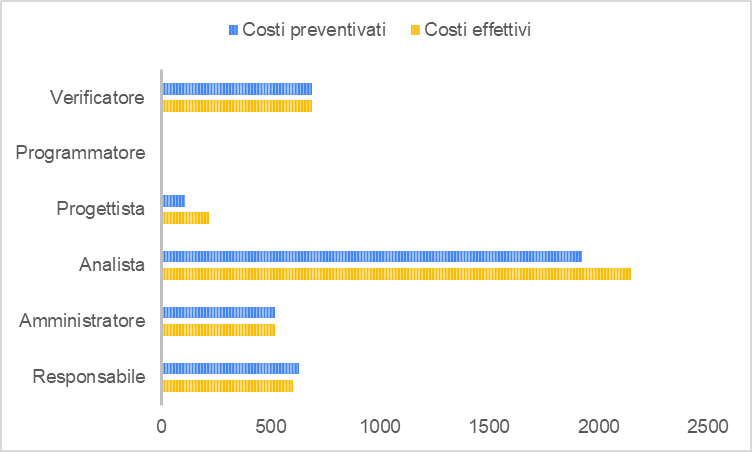
\includegraphics[width=\linewidth]{./img/Grafici/14.png}
		\caption{Grafico dei costi preventivati rispetto ai costi effettivi}
	\end{figure}

		\subsubsection{Conclusioni}
		Il bilancio risulta negativo perché le ore effettivamente svolte nei ruoli di analista, progettista e verificatore hanno superato le ore previste dal preventivo.
		Le motivazioni che hanno portato alla necessità di lavorare più del previsto sono le seguenti:
		\begin{itemize}
			\item \textbf{Analisiti}: la stesura dell'\textit{Analisi dei Requisiti} è risultata più complessa del previsto in particolare nell'individuazione dei casi d'uso\glosp e dei requisiti;
			\item \textbf{Progettisti}: sono sorte complicazioni non preventivate nella stesura del \textit{Piano di Qualifica} che hanno portato alla necessità di svolgere maggiore attività di autoapprendimento e ad un conseguente rallentamento del lavoro.
		\end{itemize}
		\subsubsection{Preventivo a finire}
		Il periodo di analisi è da intendersi come periodo di investimento per il gruppo e non viene quindi rendicontato, nel budget finale la variazione tra le ore previste e le ore effettive non provocherà alcun cambiamento. 
		È stato inoltre deciso di non modificare i successivi prospetti orari in quanto le condizioni che hanno portato alla necessità di lavorare più di quanto preventivato non dovrebbero presentarsi nuovamente. Il gruppo si ritiene ora più consapevole e meglio preparato, grazie anche alle ore di autoapprendimento già effettuate, e continua a considerare ragionevoli i prospetti orari dei prossimi periodi.
		
		\pagebreak
		\subsection{Periodo di progettazione architetturale}
		La tabella riporta il numero di ore effettivamente svolte dal gruppo e il rispettivo costo con le eventuali differenze rilevate rispetto al preventivo
		\begin{longtable} {							
				>{}p{40mm}  
				>{}p{20mm}	
				>{}p{28mm}			
			}			
			\rowcolor{gray!50}
			
			\textbf{Ruolo} & \textbf{Ore} & \textbf{Costo} \TBstrut \\
			Responsabile & 14(+1) & 420\euro (+30\euro) \TBstrut \\
			Amministratore & 13(+3) & 260\euro (+60\euro)\TBstrut \\
			Analista & 22(-2) & 550\euro (-50\euro) \TBstrut \\
			Progettista & 38 & 836\euro \TBstrut \\
			Programmatore & 58(+7) & 870\euro (+105\euro) \TBstrut \\
			Verificatore & 60 & 900\euro \TBstrut \\
			\textbf{Totale Preventivo} & 196 & 3691\euro	\TBstrut \\	
			\textbf{Totale Consuntivo} & 205 & 3836\euro	\TBstrut \\	
			\textbf{Differenza Totale} & +9 & +145\euro \TBstrut \\
			\rowcolor{white}
			\caption{Numero di ore effettivamente svolte con rispettivo costo e differenze rispetto al preventivo}	
		\end{longtable}
		Rappresentate anche dai grafici:
		\begin{figure} [H]
			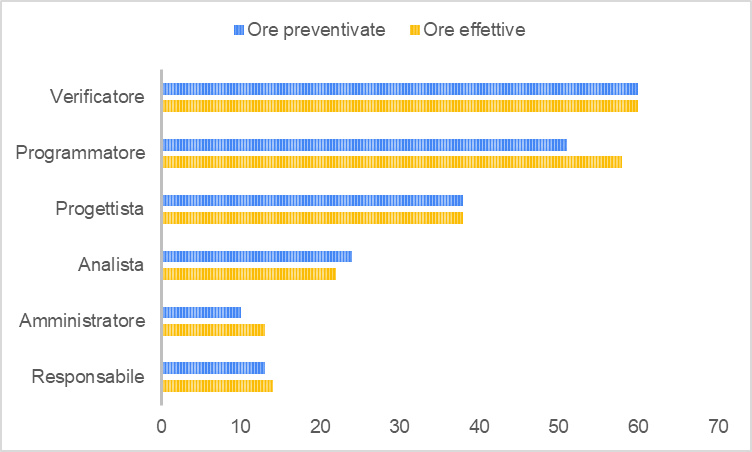
\includegraphics[width=\linewidth]{./img/Grafici/15.png}
			\caption{Grafico delle ore preventivate rispetto alle ore effettive}
		\end{figure}
		
		\begin{figure} [H]
			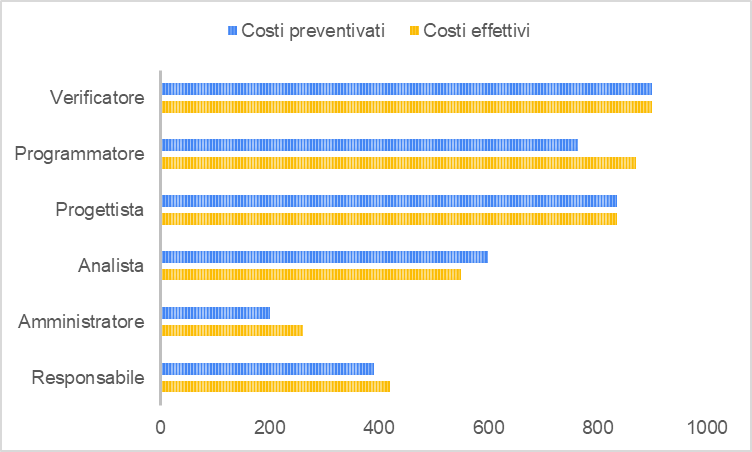
\includegraphics[width=\linewidth]{./img/Grafici/16.png}
			\caption{Grafico dei costi preventivati rispetto ai costi effettivi}
		\end{figure}
		\subsubsection{Analisi degli scostamenti}
		Al fine di garantire uno sviluppo del progetto\glosp congruo con quanto preventivato nei tempi e nei costi, al termine di ogni periodo individuato nella pianificazione si rilevano eventuali problemi riscontrati ed eventualmente si modifica e si dettaglia ulteriormente la pianificazione futura in modo da mitigare gli effetti di questi imprevisti.
		\paragraph*{I periodo} \mbox{} \\
		Il tempo dedicato alla revisione e all'aggiornamento delle \textit{Norme di Progetto} è risultato insufficiente, è stato quindi necessario prolungare quest'attività anche per il secondo periodo.
		Ciò ha causato un aumento delle ore del ruolo dell'amministratore.
		\paragraph*{II periodo} \mbox{} \\
		Al termine del secondo periodo non è stata individuata nessuna complicazione. Nonostante si sia dovuta rivedere la pianificazione vista la necessità di inserire anche in questo periodo l'attività di revisione e aggiornamento delle \textit{Norme di Progetto}, non sono stati rilevati ritardi o imprevisti oltre all'aumento delle ore per il ruolo dell'amministratore come già indicato. È stata quindi mantenuta la pianificazione prevista per il III periodo.
		\paragraph*{III periodo} \mbox{} \\
		È stato rilevato che l'attività di ricerca di strumenti e tecnologie svolta nel I periodo non è stata affiancata da un sufficiente studio degli strumenti e delle tecnologie individuate. Questo ha portato alla necessità di svolgere dell'autoapprendimento da parte di due componenti del gruppo che hanno poi illustrato quanto appreso agli altri membri. Di conseguenza si è verificato un ritardo nel ruolo dei programmatori. Questo ritardo, tuttavia, non è stato così rilevante da non permettere la codifica del Proof of Concept\glosp come da pianificazione, non è stato quindi necessario nessun cambiamento sulla pianificazione futura. 
		\paragraph*{IV periodo} \mbox{} \\
		Grazie all'attività di autoapprendimento svolta nel III periodo non ci sono stati problemi o ritardi nel IV periodo.
		\paragraph*{V periodo} \mbox{} \\
		Non sono stati rilevati scostamenti dalla pianificazione del V periodo.
		\subsubsection{Conclusioni}
		Il bilancio risulta negativo perché le ore effettivamente svolte nei ruoli di responsabile, amministratore e programmatore hanno superato le ore previste dal preventivo.
		Le motivazioni che hanno portato alla necessità di lavorare più del previsto sono le seguenti:
		\begin{itemize}
			\item \textbf{Responsabile}: per cause esterne all'ambito universitario è stato impossibile svolgere alcuni incontri previsti ed è stata necessaria una conseguente riorganizzazione delle modalità di incontro, ciò ha portato ad un inatteso aumento del lavoro per il responsabile;
			\item \textbf{Amministratore}: è sorta la necessità di utilizzare strumenti e tecnologie inizialmente non previsti, la necessità di normare l'utilizzo di quest'ultimi ha rallentato la revisione e l'aggiornamento delle \textit{Norme di Progetto} richiedendo un aumento delle ore lavorative per l'amministratore;
			\item \textbf{Programmatore}: è stato necessario uno studio più approfondito delle tecnologie rispetto a quanto non era già stato preventivato, ciò ha causato la necessità di un numero maggiore di ore anche per i programmatori.
		\end{itemize}
		Le contromisure attuate per mitigare i problemi riscontrati sono indicate nell'analisi degli scostamenti e nelle tabelle di attuazione dei rischi.
		\subsubsection{Preventivo a finire}
		Il bilancio risulta negativo in quanto i costi che abbiamo effettivamente rilevato superano quelli che erano stati preventivati. Per fronteggiare questo problema abbiamo deciso di modificare la pianificazione dei prossimi periodi in modo da presentarci ai proponenti con un preventivo finale non superiore a quello iniziale.




		
\pagebreak
\subsection{Periodo di progettazione di dettaglio e codifica}
La tabella riporta il numero di ore effettivamente svolte dal gruppo e il rispettivo costo con le eventuali differenze rilevate rispetto al preventivo
\begin{longtable} {							
		>{}p{96mm}  
		>{}p{16mm}
		>{}p{16mm}			
	}			
	\rowcolor{gray!50}
	
	\textbf{Ruolo}            & \textbf{Ore} & \textbf{Costo}       \TBstrut \\
	Responsabile              & 25           & 750\euro             \TBstrut \\
	Amministratore            & 10           & 200\euro             \TBstrut \\
	Analista                  & 19           & 475\euro             \TBstrut \\
	Progettista               & 142          & 3124\euro            \TBstrut \\
	Programmatore             & 117          & 1755\euro            \TBstrut \\
	Verificatore              & 57           & 855\euro             \TBstrut \\
	\textbf{Totale Preventivo}& 378          & 7305\euro            \TBstrut \\	
	\textbf{Totale Consuntivo}& 370          & 7159\euro            \TBstrut \\	
	\textbf{Differenza Totale rispetto alla pianificazione aggiornata}& -1          & -1\euro              \TBstrut \\
	\textbf{Differenza Totale rispetto alla pianificazione iniziale}& -8           & -146\euro              \TBstrut \\
	\rowcolor{white}
	\caption{Numero di ore effettivamente svolte con rispettivo costo e differenze rispetto al preventivo}	
\end{longtable}

Rappresentate anche dai grafici:
\begin{figure} [H]
	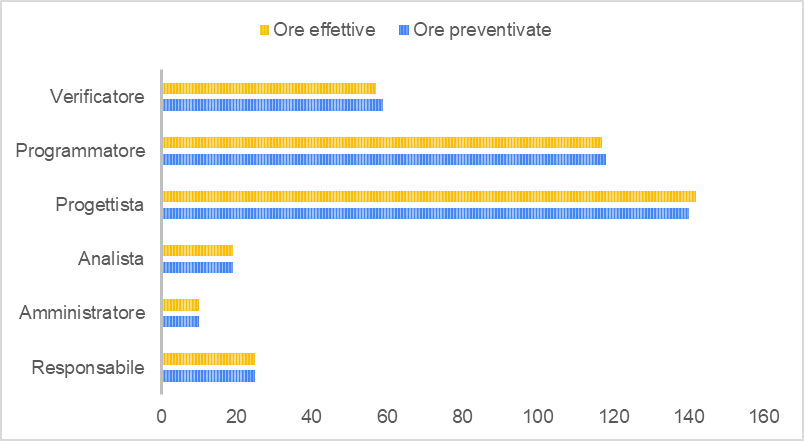
\includegraphics[width=\linewidth]{./img/Grafici/29.png}
	\caption{Grafico delle ore preventivate rispetto alle ore effettive}
\end{figure}

\begin{figure} [H]
	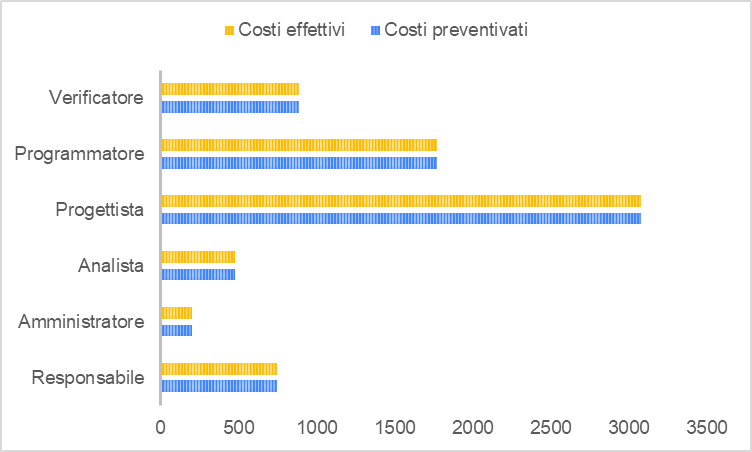
\includegraphics[width=\linewidth]{./img/Grafici/30.png}
	\caption{Grafico dei costi preventivati rispetto ai costi effettivi}
\end{figure}


\subsubsection{Conclusioni generali}
Il bilancio risulta positivo perché l'aggiornamento della pianificazione svolto in seguito al precedente consuntivo di periodo ci ha permesso di recuperare le ore in eccesso del periodo precedente.
\subsubsection{Preventivo a finire generale}
Le modifiche apportate alla pianificazione ci hanno permesso di avere un bilancio totale in pari. Questo ci permette di presentarci ai proponenti con un preventivo finale non superiore a quello iniziale.

\subsubsection{Analisi dei singoli incrementi}
Di seguito viene riportata l'analisi dell'andamento del progetto\glo. Al termine di ogni incremento individuato nella pianificazione, è stato svolto un consuntivo di periodo per poter monitorare la situazione ed eventualmente apportare delle modifiche ai periodi successivi in modo da presentarci ai proponenti con un preventivo finale non peggiore di quanto pianificato.
\paragraph{Incremento 3} \mbox{} \\
Questo incremento prevede lo sviluppo dell'algortimo di addestramento SVM\glo. \\
La tabella riporta il numero di ore effettivamente svolte dal gruppo e il rispettivo costo con le eventuali differenze rilevate rispetto al preventivo.
\begin{longtable} {							
		>{}p{40mm}  
		>{}p{20mm}	
		>{}p{28mm}			
	}			
	\rowcolor{gray!50}
	
	\textbf{Ruolo}            & \textbf{Ore} & \textbf{Costo}       \TBstrut \\
	Responsabile              & 5            & 150\euro             \TBstrut \\
	Amministratore            & 2            & 40\euro              \TBstrut \\
	Analista                  & 10           & 250\euro             \TBstrut \\
	Progettista               & 51(+1)       & 1122\euro(+22\euro)  \TBstrut \\
	Programmatore             & 32           & 480\euro             \TBstrut \\
	Verificatore              & 16(-2)       & 240\euro(-30\euro)   \TBstrut \\
	\textbf{Totale Preventivo}& 117          & 2290\euro            \TBstrut \\	
	\textbf{Totale Consuntivo}& 116          & 2282\euro            \TBstrut \\	
	\textbf{Differenza Totale}& -1           & -8\euro              \TBstrut \\
	\rowcolor{white}
	\caption{Numero di ore effettivamente svolte con rispettivo costo e differenze rispetto al preventivo}	
\end{longtable}

Rappresentate anche dai grafici:
\begin{figure} [H]
	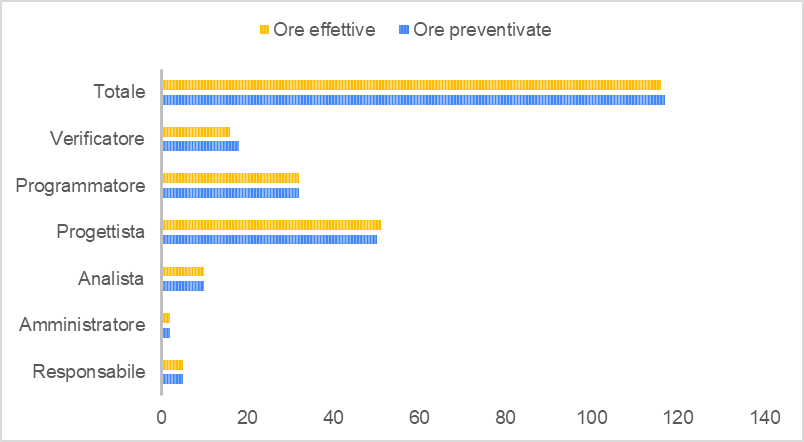
\includegraphics[width=\linewidth]{./img/Grafici/31.png}
	\caption{Grafico delle ore preventivate rispetto alle ore effettive}
\end{figure}

\begin{figure} [H]
	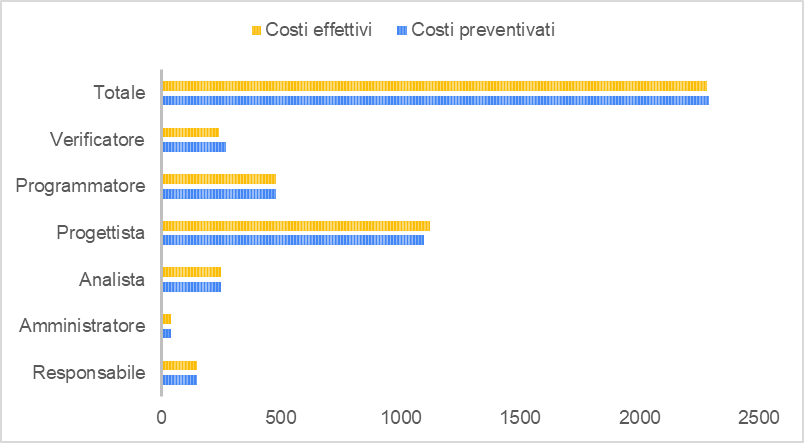
\includegraphics[width=\linewidth]{./img/Grafici/32.png}
	\caption{Grafico dei costi preventivati rispetto ai costi effettivi}
\end{figure}

\paragraph*{Analisi degli scostamenti} \mbox{} \\
Il bilancio risulta positivo perché le ore effettivamente svolte nei ruoli di progettista sono state minori di quelle previste dal preventivo, mentre, al contrario, le ore effettivamente svolte nei ruoli di verificatore sono state meno di quelle previste dal preventivo.
Le motivazioni che hanno portato a queste variazioni sono le seguenti:
\begin{itemize}
	\item \textbf{Progettista}: lo studio dell'architettura software è stata più complessa del previsto in particolare per quanto riguarda l'individuazione dei pattern architetturali;
	\item \textbf{Verificatore}: il rallentamento dello studio dell'architettura software ha portato ad avere meno materiale da verificare in questo periodo e quindi meno lavoro per i verificatori.
\end{itemize}

\paragraph*{Preventivo a finire} \mbox{} \\
Il bilancio risulta positivo in quanto i costi che abbiamo effettivamente rilevato sono inferiori a quelli che erano stati preventivati. Il denaro risparmiato è tenuto da parte per far fronte ad eventuali ritardi o per implementare i requisiti opzionali nei prossimi periodi.


\paragraph{Incremento 4}  \mbox{} \\
Questo incremento prevede lo sviluppo dell'algoritmo di addestramento RL\glo. \\
La tabella riporta il numero di ore effettivamente svolte dal gruppo e il rispettivo costo con le eventuali differenze rilevate rispetto al preventivo.
\begin{longtable} {							
		>{}p{40mm}  
		>{}p{20mm}	
		>{}p{28mm}			
	}			
	\rowcolor{gray!50}
	
	\textbf{Ruolo}            & \textbf{Ore} & \textbf{Costo}       \TBstrut \\
	Responsabile              & 4            & 120\euro             \TBstrut \\
	Amministratore            & 1            & 20\euro              \TBstrut \\
	Analista                  & 9            & 225\euro             \TBstrut \\
	Progettista               & 18(-2)       & 396\euro(-44\euro)   \TBstrut \\
	Programmatore             & 32           & 480\euro             \TBstrut \\
	Verificatore              & 17           & 255\euro             \TBstrut \\
	\textbf{Totale Preventivo}& 83           & 1540\euro            \TBstrut \\	
	\textbf{Totale Consuntivo}& 81           & 1496\euro            \TBstrut \\	
	\textbf{Differenza Totale}& -2           & -44\euro             \TBstrut \\
	\rowcolor{white}
	\caption{Numero di ore effettivamente svolte con rispettivo costo e differenze rispetto al preventivo}	
\end{longtable}

Rappresentate anche dai grafici:
\begin{figure} [H]
	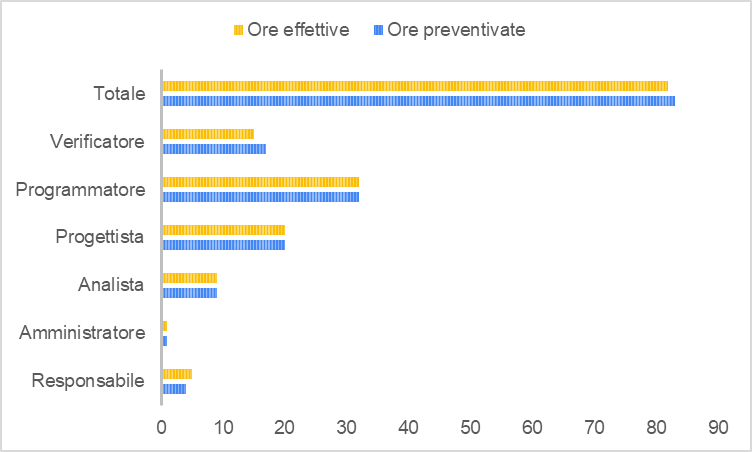
\includegraphics[width=\linewidth]{./img/Grafici/33.png}
	\caption{Grafico delle ore preventivate rispetto alle ore effettive}
\end{figure}

\begin{figure} [H]
	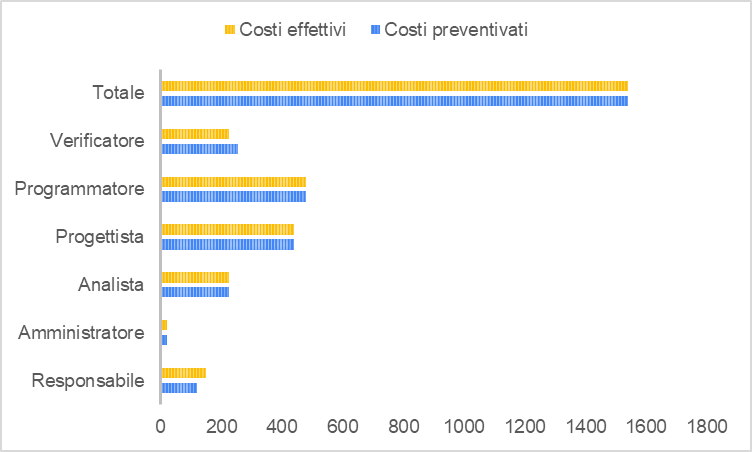
\includegraphics[width=\linewidth]{./img/Grafici/34.png}
	\caption{Grafico dei costi preventivati rispetto ai costi effettivi}
\end{figure}

\paragraph*{Analisi degli scostamenti} \mbox{} \\
Il bilancio risulta in pari perché, sebbene le ore totali svolte siano inferiori a quanto presente nel preventivo, le ore nei ruoli di responsabile hanno superato quelle preventivate. Al contrario, le ore effettivamente svolte nei ruoli di verificatore sono state meno di quelle previste dal preventivo.
Le motivazioni che hanno portato a queste variazioni sono le seguenti:
\begin{itemize}
	\item \textbf{Progettista}: in seguito al maggior lavoro svolto dal progettista nel periodo precedente, è stato necessario un minor impegno orario per far fronte lo sviluppo dell'incremento 4 in quanto alcuni componenti erano già parzialmente strutturati.
\end{itemize}

\paragraph*{Preventivo a finire} \mbox{} \\
Il bilancio risulta positivo in quanto i costi che abbiamo effettivamente rilevato sono minori di quelli che erano stati preventivati. Per questo non è necessario modificare i preventivi dei periodi rimanenti mentre le risorse risparmiate vengono mantenute per sopperire ad eventuali rallentamenti che potrebbero sorgere o per implementare i requisiti opzionali.



\paragraph{Incremento 6}  \mbox{} \\
Questo incremento prevede lo sviluppo della selezione del modello di addestramento da applicare e del suo avvio. \\
La tabella riporta il numero di ore effettivamente svolte dal gruppo e il rispettivo costo con le eventuali differenze rilevate rispetto al preventivo.
\begin{longtable} {							
		>{}p{40mm}  
		>{}p{20mm}	
		>{}p{28mm}			
	}			
	\rowcolor{gray!50}
	
	\textbf{Ruolo}            & \textbf{Ore} & \textbf{Costo}       \TBstrut \\
	Responsabile              & 4            & 120\euro    \TBstrut \\
	Amministratore            & 2            & 40\euro              \TBstrut \\
	Analista                  & 0            & 0\euro               \TBstrut \\
	Progettista               & 20           & 440\euro             \TBstrut \\
	Programmatore             & 10           & 150\euro             \TBstrut \\
	Verificatore              & 4            & 60\euro              \TBstrut \\
	\textbf{Totale Preventivo}& 40           & 810\euro             \TBstrut \\	
	\textbf{Totale Consuntivo}& 40           & 810\euro             \TBstrut \\	
	\textbf{Differenza Totale}& 0            & 0\euro             \TBstrut \\
	\rowcolor{white}
	\caption{Numero di ore effettivamente svolte con rispettivo costo e differenze rispetto al preventivo}	
\end{longtable}

Rappresentate anche dai grafici:
\begin{figure} [H]
	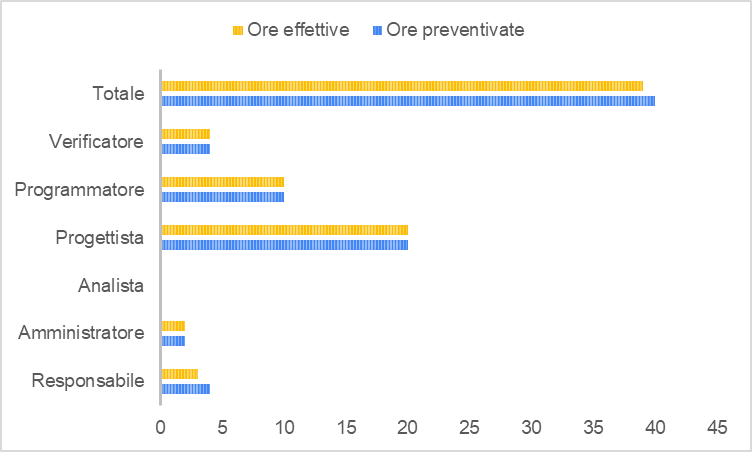
\includegraphics[width=\linewidth]{./img/Grafici/35.png}
	\caption{Grafico delle ore preventivate rispetto alle ore effettive}
\end{figure}

\begin{figure} [H]
	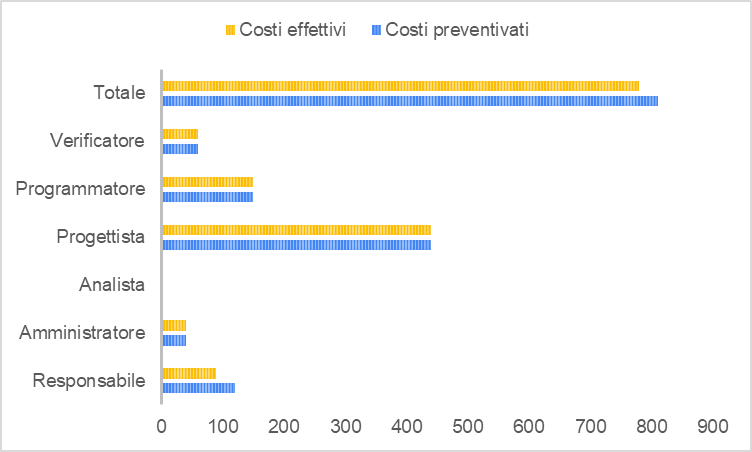
\includegraphics[width=\linewidth]{./img/Grafici/36.png}
	\caption{Grafico dei costi preventivati rispetto ai costi effettivi}
\end{figure}

\paragraph*{Analisi degli scostamenti} \mbox{} \\
Il bilancio risulta in pari in quanto i costi che abbiamo effettivamente rilevato eguagliano quelli che erano stati preventivati. In questo periodo infatti non è sorta nessuna problematica.


\paragraph*{Preventivo a finire} \mbox{} \\
Il bilancio risulta in pari in quanto i costi che abbiamo effettivamente rilevato eguagliano quelli che erano stati preventivati; non è quindi necessaria alcuna modifica alla pianificazione degli incrementi futuri.



\paragraph{Incremento 13} \mbox{} \\
Questo incremento prevede lo sviluppo della lettura del file JSON e della configurazione degli algoritmi nel plug-in. \\
La tabella riporta il numero di ore effettivamente svolte dal gruppo e il rispettivo costo con le eventuali differenze rilevate rispetto al preventivo.
\begin{longtable} {							
		>{}p{40mm}  
		>{}p{20mm}	
		>{}p{28mm}			
	}			
	\rowcolor{gray!50}
	
	\textbf{Ruolo}            & \textbf{Ore} & \textbf{Costo}       \TBstrut \\
	Responsabile              & 4            & 120\euro    \TBstrut \\
	Amministratore            & 2            & 40\euro              \TBstrut \\
	Analista                  & 0            & 0\euro               \TBstrut \\
	Progettista               & 11(+1)       & 242\euro(+22\euro)   \TBstrut \\
	Programmatore             & 8            & 120\euro             \TBstrut \\
	Verificatore              & 3            & 45\euro              \TBstrut \\
	\textbf{Totale Preventivo}& 27           & 545\euro             \TBstrut \\	
	\textbf{Totale Consuntivo}& 28           & 567\euro             \TBstrut \\	
	\textbf{Differenza Totale}& +1           & +22\euro              \TBstrut \\
	\rowcolor{white}
	\caption{Numero di ore effettivamente svolte con rispettivo costo e differenze rispetto al preventivo}	
\end{longtable}

Rappresentate anche dai grafici:
\begin{figure} [H]
	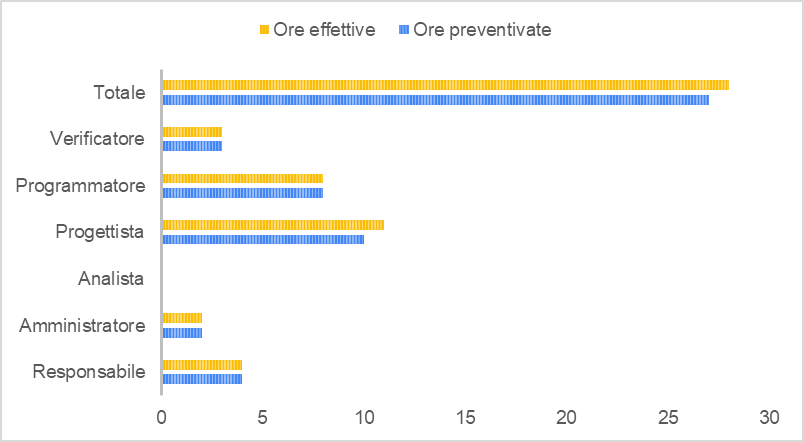
\includegraphics[width=\linewidth]{./img/Grafici/37.png}
	\caption{Grafico delle ore preventivate rispetto alle ore effettive}
\end{figure}

\begin{figure} [H]
	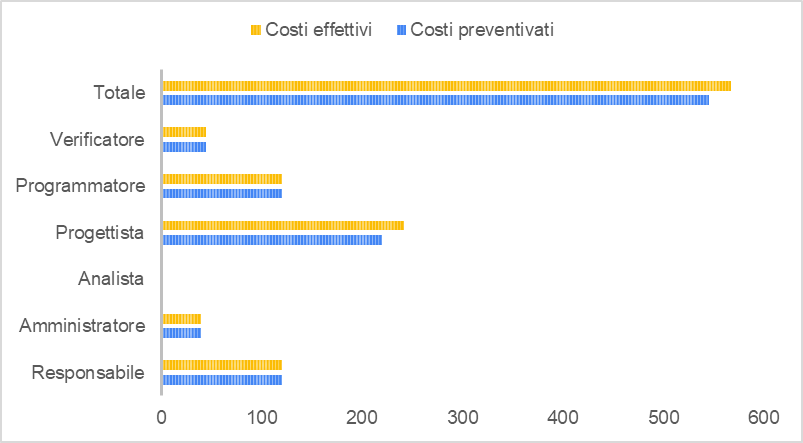
\includegraphics[width=\linewidth]{./img/Grafici/38.png}
	\caption{Grafico dei costi preventivati rispetto ai costi effettivi}
\end{figure}

\paragraph*{Analisi degli scostamenti} \mbox{} \\
Il bilancio risulta negativo perché le ore effettivamente svolte nel ruolo di progettista sono state maggiori rispetto a quelle previste dal preventivo.
Le motivazioni che hanno portato a queste variazioni sono le seguenti:
\begin{itemize}
	\item \textbf{Progettista}: la lezione sui design pattern e la risposta del committente prof. Cardin hanno portato i progettisti a cambiare parte della struttura del lavoro svolto fino a quel momento ed è stato quindi necessario un impegno orario maggiore di quanto preventivato.
\end{itemize}

\paragraph*{Preventivo a finire} \mbox{} \\
Il bilancio risulta negativo in quanto i costi che abbiamo effettivamente rilevato sono superiori a quelli che erano stati preventivati. Il denaro impiegato in più non verrà fatto risultare nel preventivo a finire in quanto verrà preso da ciò che è stato risparmiato nei periodi precedenti.


\paragraph{Incremento 14} \mbox{} \\
Questo incremento prevede lo sviluppo dell'associazione dei nodi al flusso dati all'interno del plug-in Grafana\glo. \\ 
La tabella riporta il numero di ore effettivamente svolte dal gruppo e il rispettivo costo con le eventuali differenze rilevate rispetto al preventivo.
\begin{longtable} {							
		>{}p{40mm}  
		>{}p{20mm}	
		>{}p{28mm}			
	}			
	\rowcolor{gray!50}
	
	\textbf{Ruolo}            & \textbf{Ore} & \textbf{Costo}       \TBstrut \\
	Responsabile              & 4            & 120\euro             \TBstrut \\
	Amministratore            & 2            & 40\euro              \TBstrut \\
	Analista                  & 0            & 0\euro               \TBstrut \\
	Progettista               & 34(+4)       & 748\euro             \TBstrut \\
	Programmatore             & 27(-1)       & 405\euro(-30\euro)   \TBstrut \\
	Verificatore              & 14           & 210\euro             \TBstrut \\
	\textbf{Totale Preventivo}& 78           & 1450\euro            \TBstrut \\	
	\textbf{Totale Consuntivo}& 81           & 1523\euro            \TBstrut \\	
	\textbf{Differenza Totale}& +3           & +73\euro             \TBstrut \\
	\rowcolor{white}
	\caption{Numero di ore effettivamente svolte con rispettivo costo e differenze rispetto al preventivo}	
\end{longtable}

Rappresentate anche dai grafici:
\begin{figure} [H]
	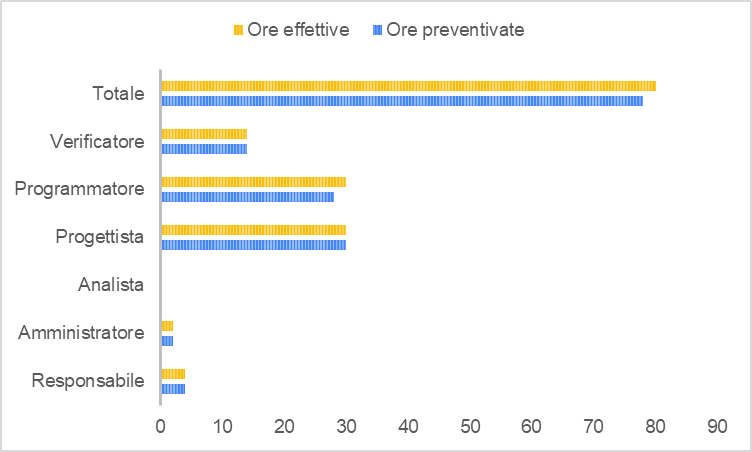
\includegraphics[width=\linewidth]{./img/Grafici/39.png}
	\caption{Grafico delle ore preventivate rispetto alle ore effettive}
\end{figure}

\begin{figure} [H]
	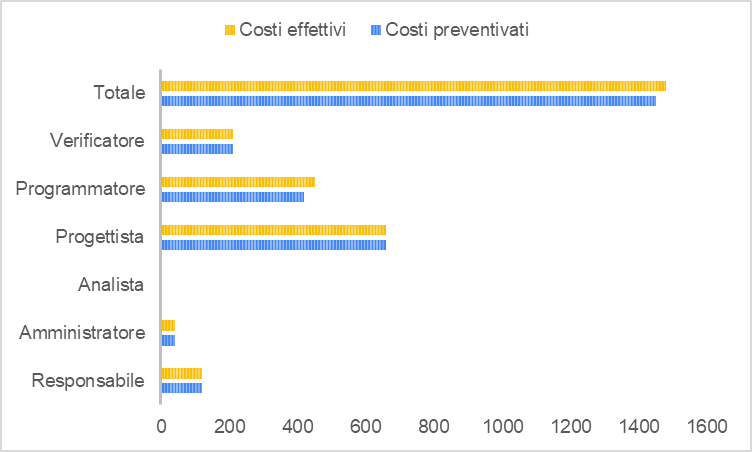
\includegraphics[width=\linewidth]{./img/Grafici/40.png}
	\caption{Grafico dei costi preventivati rispetto ai costi effettivi}
\end{figure}

\paragraph*{Analisi degli scostamenti} \mbox{} \\
Il bilancio risulta negativo perché le ore effettivamente svolte nei ruoli di programmatore sono state maggiori rispetto a quelle previste dal preventivo.
Le motivazioni che hanno portato a queste variazioni sono le seguenti:
\begin{itemize}
	\item \textbf{Progettista}: in seguito alla presentazione della Product Baseline, il committente prof. Cardin ha segnalato alcuni errori ed è quindi sorta la necessità di modificare alcune parti dell'architettura. Per questo motivo è stato necessario un impegno orario maggiore da parte del progettista.
\end{itemize}
\paragraph*{Preventivo a finire} \mbox{} \\
Il bilancio risulta negativo in quanto i costi che abbiamo effettivamente rilevato sono superiori a quelli che erano stati preventivati. Per fronteggiare questo problema abbiamo deciso di modificare la pianificazione dei prossimi periodi, andando a ridurre le ore del progettista, in modo da presentarci ai proponenti con un preventivo finale in linea con quello iniziale. In questo ci aiuta il fatto che nei periodi precedenti abbiamo speso meno di quanto preventivato.


\paragraph{Incremento 16} \mbox{} \\
Questo incremento prevede lo sviluppo dell'arresto del plug-in prima della sua naturale conclusione. \\
La tabella riporta il numero di ore effettivamente svolte dal gruppo e il rispettivo costo con le eventuali differenze rilevate rispetto al preventivo.
\begin{longtable} {							
		>{}p{40mm}  
		>{}p{20mm}	
		>{}p{28mm}			
	}			
	\rowcolor{gray!50}
	
	\textbf{Ruolo}            & \textbf{Ore} & \textbf{Costo}       \TBstrut \\
	Responsabile              & 4            & 120\euro             \TBstrut \\
	Amministratore            & 1            & 20\euro              \TBstrut \\
	Analista                  & 0            & 0\euro               \TBstrut \\
	Progettista               & 8(-2)        & 176\euro(-44\euro)   \TBstrut \\
	Programmatore             & 8            & 120\euro             \TBstrut \\
	Verificatore              & 3            & 45\euro              \TBstrut \\
	\textbf{Totale Preventivo}& 26           & 525\euro             \TBstrut \\	
	\textbf{Totale Consuntivo}& 24           & 481\euro             \TBstrut \\	
	\textbf{Differenza Totale}& -2           & -44\euro             \TBstrut \\
	\rowcolor{white}
	\caption{Numero di ore effettivamente svolte con rispettivo costo e differenze rispetto al preventivo}	
\end{longtable}

Rappresentate anche dai grafici:
\begin{figure} [H]
	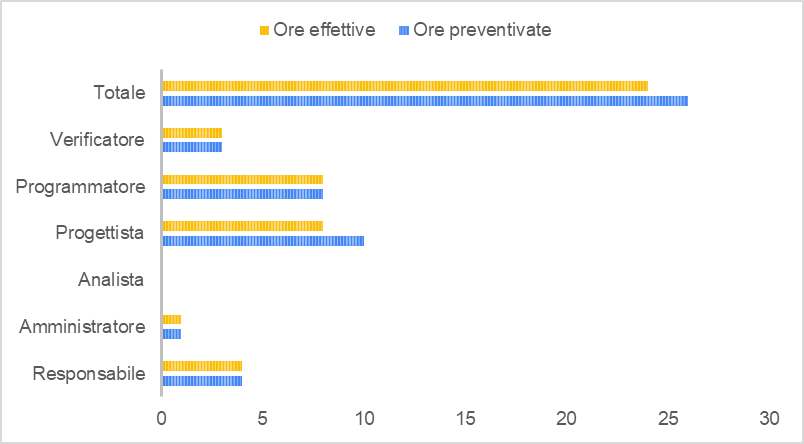
\includegraphics[width=\linewidth]{./img/Grafici/41.png}
	\caption{Grafico delle ore preventivate rispetto alle ore effettive}
\end{figure}

\begin{figure} [H]
	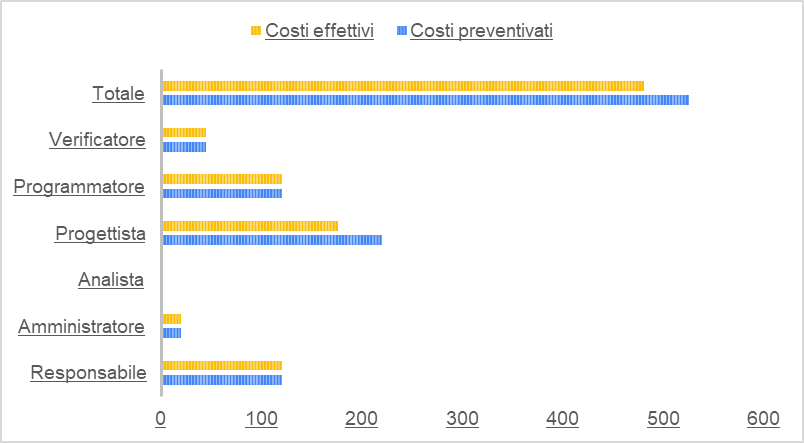
\includegraphics[width=\linewidth]{./img/Grafici/42.png}
	\caption{Grafico dei costi preventivati rispetto ai costi effettivi}
\end{figure}

\paragraph*{Analisi degli scostamenti} \mbox{} \\
Il bilancio risulta positivo perché le ore effettivamente svolte nei ruolo di progettista sono state inferiori rispetto a quelle previste dal preventivo,
Le motivazioni che hanno portato a queste variazioni sono le seguenti:
\begin{itemize}
	\item \textbf{progettista}: il lavoro in più svolto nei precedenti periodi ha portato a meno lavoro per il progettista.
\end{itemize}
\paragraph*{Preventivo a finire} \mbox{} \\
Il bilancio risulta positivo in quanto i costi che abbiamo effettivamente rilevato sono inferiori a quelli che erano stati preventivati. Questi soldi risparmiati vengono utilizzati per coprire le spese in eccesso del periodo precedente.









































